\section{Messwerte und Auswertung}
\label{sec:messwerte}
	
	\subsection{Abschätzung der oberen Strahlendosis}
	\label{ssec:strahlendosis}
	
		Für die Abschätzung soll angenommen werden, dass wir uns für circa $t = 12\unit{h}$ in einem Abstand von $r = 1\unit{m}$ zu einer $\prescript{60}{}{\m{Co}}$- beziehungsweise einer $\prescript{137}{}{\m{Cs}}$-Quelle befinden.
		Diese Quellen besitzen in etwa eine Aktivität von $A = 200\unit{kBq}$.
		Für die Proportionalitätsfaktoren ergeben sich
		\begin{alignat*}{3}
			\Gamma_H\curvb{ \prescript{60}{}{\m{Co}} } &=&\ 351 \unit{\mu Sv\, m^2 \, \inv{h} \, \inv{GBq}} \\
			\Gamma_H\curvb{ \prescript{137}{}{\m{Cs}} } &=&\ 88 \unit{\mu Sv\, m^2 \, \inv{h} \, \inv{GBq}}
		\end{alignat*}
		Die aufgenommene Äquivalentdosis ist gerade durch folgende Gleichung gegeben.
		\[
			H = \Gamma_H A t r^2
		\]
		\[
			\implies \quad H_\m{Co} = 0.84 \unit{\mu Sv},\qquad H_\m{Cs} = 0.12 \unit{\mu Sv}
		\]
		Die in der gleichen Zeit durch die Umgebung abgegebene Strahlungsdosis beträgt ungefähr $5.48\unit{\mu Sv}$ und beträgt damit ein Vielfaches der errechneten Werte.
	
	% subsection strahlendosis

	\FloatBarrier
	\subsection{Messung eines $\gamma$-Spektrums}
	\label{ssec:gamma-spektrum}

		Für die Aufnahme der $\gamma$-Spektren gab es drei wesentliche Parameter.
		\begin{itemize}
			\item $d\ldots$ Abstand der Quelle vom Detektor
			\item $t_\m{real}\ldots$ gesamte Aufnahmezeit eines $\gamma$-Spektrums
			\item $t_\m{live}\ldots$ effektive Aufnahmezeit: Differenz aus Aufnahmezeit und Totzeit$_\skull$
		\end{itemize}
		Die hier eingeführten Formelzeichen und Bezeichnungen sollen auch im Folgenden verwendet werden.
		Um die Funktionsweise des Detektors und des Vielkanalanalysator anschaulich zu machen, wurde zunächst das Spektrum einer $\prescript{22}{}{\m{Na}}$-Quelle aufgenommen und in Abbildung \ref{fig:na-22-spec-1} dargestellt. 
	
		\begin{figure}[htb]
			\centering
			% GNUPLOT: LaTeX picture with Postscript
\begingroup
  \makeatletter
  \providecommand\color[2][]{%
    \GenericError{(gnuplot) \space\space\space\@spaces}{%
      Package color not loaded in conjunction with
      terminal option `colourtext'%
    }{See the gnuplot documentation for explanation.%
    }{Either use 'blacktext' in gnuplot or load the package
      color.sty in LaTeX.}%
    \renewcommand\color[2][]{}%
  }%
  \providecommand\includegraphics[2][]{%
    \GenericError{(gnuplot) \space\space\space\@spaces}{%
      Package graphicx or graphics not loaded%
    }{See the gnuplot documentation for explanation.%
    }{The gnuplot epslatex terminal needs graphicx.sty or graphics.sty.}%
    \renewcommand\includegraphics[2][]{}%
  }%
  \providecommand\rotatebox[2]{#2}%
  \@ifundefined{ifGPcolor}{%
    \newif\ifGPcolor
    \GPcolorfalse
  }{}%
  \@ifundefined{ifGPblacktext}{%
    \newif\ifGPblacktext
    \GPblacktexttrue
  }{}%
  % define a \g@addto@macro without @ in the name:
  \let\gplgaddtomacro\g@addto@macro
  % define empty templates for all commands taking text:
  \gdef\gplbacktext{}%
  \gdef\gplfronttext{}%
  \makeatother
  \ifGPblacktext
    % no textcolor at all
    \def\colorrgb#1{}%
    \def\colorgray#1{}%
  \else
    % gray or color?
    \ifGPcolor
      \def\colorrgb#1{\color[rgb]{#1}}%
      \def\colorgray#1{\color[gray]{#1}}%
      \expandafter\def\csname LTw\endcsname{\color{white}}%
      \expandafter\def\csname LTb\endcsname{\color{black}}%
      \expandafter\def\csname LTa\endcsname{\color{black}}%
      \expandafter\def\csname LT0\endcsname{\color[rgb]{1,0,0}}%
      \expandafter\def\csname LT1\endcsname{\color[rgb]{0,1,0}}%
      \expandafter\def\csname LT2\endcsname{\color[rgb]{0,0,1}}%
      \expandafter\def\csname LT3\endcsname{\color[rgb]{1,0,1}}%
      \expandafter\def\csname LT4\endcsname{\color[rgb]{0,1,1}}%
      \expandafter\def\csname LT5\endcsname{\color[rgb]{1,1,0}}%
      \expandafter\def\csname LT6\endcsname{\color[rgb]{0,0,0}}%
      \expandafter\def\csname LT7\endcsname{\color[rgb]{1,0.3,0}}%
      \expandafter\def\csname LT8\endcsname{\color[rgb]{0.5,0.5,0.5}}%
    \else
      % gray
      \def\colorrgb#1{\color{black}}%
      \def\colorgray#1{\color[gray]{#1}}%
      \expandafter\def\csname LTw\endcsname{\color{white}}%
      \expandafter\def\csname LTb\endcsname{\color{black}}%
      \expandafter\def\csname LTa\endcsname{\color{black}}%
      \expandafter\def\csname LT0\endcsname{\color{black}}%
      \expandafter\def\csname LT1\endcsname{\color{black}}%
      \expandafter\def\csname LT2\endcsname{\color{black}}%
      \expandafter\def\csname LT3\endcsname{\color{black}}%
      \expandafter\def\csname LT4\endcsname{\color{black}}%
      \expandafter\def\csname LT5\endcsname{\color{black}}%
      \expandafter\def\csname LT6\endcsname{\color{black}}%
      \expandafter\def\csname LT7\endcsname{\color{black}}%
      \expandafter\def\csname LT8\endcsname{\color{black}}%
    \fi
  \fi
  \setlength{\unitlength}{0.0500bp}%
  \begin{picture}(7086.00,3968.00)%
    \gplgaddtomacro\gplbacktext{%
      \csname LTb\endcsname%
      \put(814,704){\makebox(0,0)[r]{\strut{}$10^0$}}%
      \put(814,1304){\makebox(0,0)[r]{\strut{}$10^1$}}%
      \put(814,1904){\makebox(0,0)[r]{\strut{}$10^2$}}%
      \put(814,2503){\makebox(0,0)[r]{\strut{}$10^3$}}%
      \put(814,3103){\makebox(0,0)[r]{\strut{}$10^4$}}%
      \put(814,3703){\makebox(0,0)[r]{\strut{}$10^5$}}%
      \put(946,484){\makebox(0,0){\strut{} 0}}%
      \put(1584,484){\makebox(0,0){\strut{} 200}}%
      \put(2222,484){\makebox(0,0){\strut{} 400}}%
      \put(2860,484){\makebox(0,0){\strut{} 600}}%
      \put(3498,484){\makebox(0,0){\strut{} 800}}%
      \put(4137,484){\makebox(0,0){\strut{} 1000}}%
      \put(4775,484){\makebox(0,0){\strut{} 1200}}%
      \put(5413,484){\makebox(0,0){\strut{} 1400}}%
      \put(6051,484){\makebox(0,0){\strut{} 1600}}%
      \put(6689,484){\makebox(0,0){\strut{} 1800}}%
      \put(176,2203){\rotatebox{-270}{\makebox(0,0){\strut{}Counts}}}%
      \put(3817,154){\makebox(0,0){\strut{}$E \ [\unit{keV}]$}}%
      \put(2956,3103){\makebox(0,0)[l]{\strut{}$\curlywedge\beta^+$}}%
      \put(4073,2785){\makebox(0,0)[l]{\strut{}$\curlywedge\prescript{22}{}{\m{Na}}$}}%
      \put(5891,2230){\makebox(0,0)[l]{\strut{}$\curlywedge\prescript{40}{}{\m{K}}$}}%
      \put(1903,1771){\makebox(0,0)[l]{\strut{}$\neg\beta^+$}}%
      \put(4137,1304){\makebox(0,0)[l]{\strut{}$\neg\prescript{22}{}{\m{Na}}$}}%
    }%
    \gplgaddtomacro\gplfronttext{%
      \csname LTb\endcsname%
      \put(5702,3420){\makebox(0,0)[r]{\strut{}Messwerte}}%
    }%
    \gplbacktext
    \put(0,0){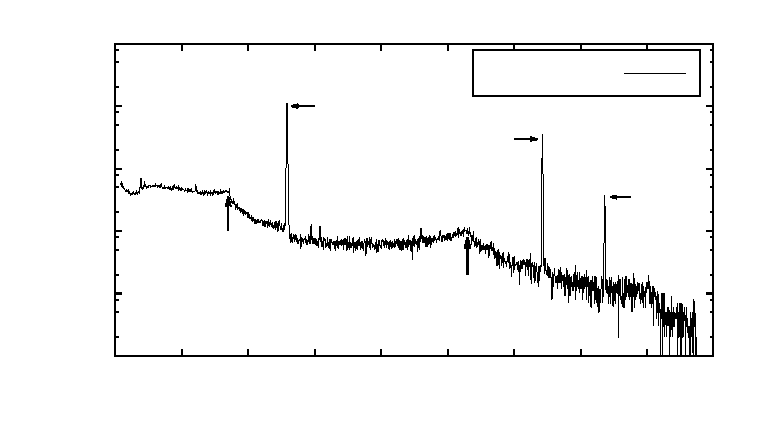
\includegraphics{na-22-spec-1}}%
    \gplfronttext
  \end{picture}%
\endgroup

			\caption{$\gamma$-Spektrum einer $\prescript{22}{}{\m{Na}}$-Quelle aufgenommen durch einen HP-Ge-Detektor. \\ Parameter: $d=0\unit{cm}$, $t_\m{live}=595\unit{s}$, $t_\m{real}=609\unit{s}$} % fick dich schröter
			\label{fig:na-22-spec-1}
		\end{figure}

		Klar zu erkennen sind die Vollabsorptionspeaks, welche im Diagramm durch $\curlywedge$ und deren Ursache beschriftet sind.
		Die genauen Werte befinden sich in Tabelle \ref{tab:na-22-peaks}.

		\urldef{\refData}\url{https://www.cpp.edu/~pbsiegel/bio431/genergies.html}
		\begin{table}[H]
			\centering
			\begin{tabular}{r||r|r|r}
				Theorie $[\unit{keV}]$ & $511$ & $1275$ & $1460$ \\
				\hline
				Messwerte $[\unit{keV}]$ & $517$ & $1285$ & $1473$ \\
			\end{tabular}
			\caption{Photopeaks des $\prescript{22}{}{\m{Na}}$-Spektrums mit Untergrund \\ Quelle: \refData}
			\label{tab:na-22-peaks}
		\end{table}

		Aus diesen Daten wird ersichtlich, dass ein systematischer Fehler auftritt, welcher auf eine fehlende Kalibrierung der Abszisse hinweist (siehe Abschnitt \ref{ssec:kalibrierung}).

		Wie aus den Grundlagen bekannt existieren zu jedem Photopeak Comptonkanten bei einer kleineren Energie.
		Im Diagramm sind diese mit $\neg$ und deren Ursache gekennzeichnet.
		Tabelle \ref{tab:na-22-compton} zeigt die gemessenen Kanten im Vergleich zu den rein theoretisch berechneten Werten (Theorie) und den aus den Messungen berechneten Werten (ber. Werte) für die Kanten.
		Zur Berechnung wurde die Formel aus Abschnitt \ref{sssec:comptoneffekt} verwendet.

		\begin{table}[H]
			\centering
			\begin{tabular}{r||r|r|r}
				Theorie $[\unit{keV}]$ & $341$ & $1062$ & $1243$ \\
				\hline
				ber. Wert $[\unit{keV}]$ & $346$ & $1072$ & $1255$ \\
				\hline
				Messwerte $[\unit{keV}]$ & $350$ & $1060$ & --- \\
			\end{tabular}
			\caption{Comptonkanten des $\prescript{22}{}{\m{Na}}$-Spektrums mit Untergrund \\ Quelle: \refData}
			\label{tab:na-22-compton}
		\end{table}

		Für eine feste Wellenlänge ist die durch den Comptoneffekt abgegebene Energie bis zur jeweiligen Comptonkante kontinuierlich verteilt.
		Im Diagramm wird dieser Effekt durch die auftretenden Stufen deutlich.
		Die Comptonkante des $\prescript{40}{}{\m{K}}$-Peaks ist aufgrund des vorhandenen Rauschens und der Überlagerung mit anderen Peaks nicht erkennbar.

		Bei jedem aufgenommenen $\gamma$-Spektrum ist zu beachten, dass man zusätzlich zum Signal des Strahlers auch noch das Signal der natürlich vorkommenden Strahlung misst.

		\begin{figure}[htb]
			\centering
			% GNUPLOT: LaTeX picture with Postscript
\begingroup
  \makeatletter
  \providecommand\color[2][]{%
    \GenericError{(gnuplot) \space\space\space\@spaces}{%
      Package color not loaded in conjunction with
      terminal option `colourtext'%
    }{See the gnuplot documentation for explanation.%
    }{Either use 'blacktext' in gnuplot or load the package
      color.sty in LaTeX.}%
    \renewcommand\color[2][]{}%
  }%
  \providecommand\includegraphics[2][]{%
    \GenericError{(gnuplot) \space\space\space\@spaces}{%
      Package graphicx or graphics not loaded%
    }{See the gnuplot documentation for explanation.%
    }{The gnuplot epslatex terminal needs graphicx.sty or graphics.sty.}%
    \renewcommand\includegraphics[2][]{}%
  }%
  \providecommand\rotatebox[2]{#2}%
  \@ifundefined{ifGPcolor}{%
    \newif\ifGPcolor
    \GPcolorfalse
  }{}%
  \@ifundefined{ifGPblacktext}{%
    \newif\ifGPblacktext
    \GPblacktexttrue
  }{}%
  % define a \g@addto@macro without @ in the name:
  \let\gplgaddtomacro\g@addto@macro
  % define empty templates for all commands taking text:
  \gdef\gplbacktext{}%
  \gdef\gplfronttext{}%
  \makeatother
  \ifGPblacktext
    % no textcolor at all
    \def\colorrgb#1{}%
    \def\colorgray#1{}%
  \else
    % gray or color?
    \ifGPcolor
      \def\colorrgb#1{\color[rgb]{#1}}%
      \def\colorgray#1{\color[gray]{#1}}%
      \expandafter\def\csname LTw\endcsname{\color{white}}%
      \expandafter\def\csname LTb\endcsname{\color{black}}%
      \expandafter\def\csname LTa\endcsname{\color{black}}%
      \expandafter\def\csname LT0\endcsname{\color[rgb]{1,0,0}}%
      \expandafter\def\csname LT1\endcsname{\color[rgb]{0,1,0}}%
      \expandafter\def\csname LT2\endcsname{\color[rgb]{0,0,1}}%
      \expandafter\def\csname LT3\endcsname{\color[rgb]{1,0,1}}%
      \expandafter\def\csname LT4\endcsname{\color[rgb]{0,1,1}}%
      \expandafter\def\csname LT5\endcsname{\color[rgb]{1,1,0}}%
      \expandafter\def\csname LT6\endcsname{\color[rgb]{0,0,0}}%
      \expandafter\def\csname LT7\endcsname{\color[rgb]{1,0.3,0}}%
      \expandafter\def\csname LT8\endcsname{\color[rgb]{0.5,0.5,0.5}}%
    \else
      % gray
      \def\colorrgb#1{\color{black}}%
      \def\colorgray#1{\color[gray]{#1}}%
      \expandafter\def\csname LTw\endcsname{\color{white}}%
      \expandafter\def\csname LTb\endcsname{\color{black}}%
      \expandafter\def\csname LTa\endcsname{\color{black}}%
      \expandafter\def\csname LT0\endcsname{\color{black}}%
      \expandafter\def\csname LT1\endcsname{\color{black}}%
      \expandafter\def\csname LT2\endcsname{\color{black}}%
      \expandafter\def\csname LT3\endcsname{\color{black}}%
      \expandafter\def\csname LT4\endcsname{\color{black}}%
      \expandafter\def\csname LT5\endcsname{\color{black}}%
      \expandafter\def\csname LT6\endcsname{\color{black}}%
      \expandafter\def\csname LT7\endcsname{\color{black}}%
      \expandafter\def\csname LT8\endcsname{\color{black}}%
    \fi
  \fi
  \setlength{\unitlength}{0.0500bp}%
  \begin{picture}(7086.00,3968.00)%
    \gplgaddtomacro\gplbacktext{%
      \csname LTb\endcsname%
      \put(814,704){\makebox(0,0)[r]{\strut{}$10^0$}}%
      \put(814,1304){\makebox(0,0)[r]{\strut{}$10^1$}}%
      \put(814,1904){\makebox(0,0)[r]{\strut{}$10^2$}}%
      \put(814,2503){\makebox(0,0)[r]{\strut{}$10^3$}}%
      \put(814,3103){\makebox(0,0)[r]{\strut{}$10^4$}}%
      \put(814,3703){\makebox(0,0)[r]{\strut{}$10^5$}}%
      \put(946,484){\makebox(0,0){\strut{} 0}}%
      \put(1584,484){\makebox(0,0){\strut{} 200}}%
      \put(2222,484){\makebox(0,0){\strut{} 400}}%
      \put(2860,484){\makebox(0,0){\strut{} 600}}%
      \put(3498,484){\makebox(0,0){\strut{} 800}}%
      \put(4137,484){\makebox(0,0){\strut{} 1000}}%
      \put(4775,484){\makebox(0,0){\strut{} 1200}}%
      \put(5413,484){\makebox(0,0){\strut{} 1400}}%
      \put(6051,484){\makebox(0,0){\strut{} 1600}}%
      \put(6689,484){\makebox(0,0){\strut{} 1800}}%
      \put(176,2203){\rotatebox{-270}{\makebox(0,0){\strut{}Counts}}}%
      \put(3817,154){\makebox(0,0){\strut{}$E \ [\unit{keV}]$}}%
    }%
    \gplgaddtomacro\gplfronttext{%
      \csname LTb\endcsname%
      \put(5702,3420){\makebox(0,0)[r]{\strut{}Messwerte}}%
    }%
    \gplbacktext
    \put(0,0){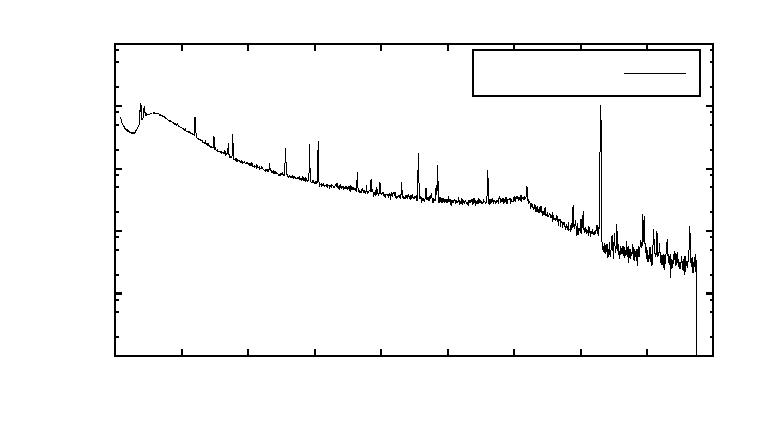
\includegraphics{back-1}}%
    \gplfronttext
  \end{picture}%
\endgroup

			\caption{natürliches $\gamma$-Spektrums aufgenommen durch einen HP-Ge-Detektor \\ Parameter: $t_\m{live}=16447\unit{s}$, $t_\m{real}=16551\unit{s}$}
			\label{fig:back-1}
		\end{figure}

		Abbildung \ref{fig:back-1} zeigt das Spektrum der natürlichen Strahlung.
		Klar zu erkennen ist wieder die $\prescript{40}{}{\m{K}}$-Linie.
		Andere auftretende Peaks stammen von anderen natürlichen Isotopen wie zum Beispiel aus der Thorium- und Uran-Reihe.
	
	% subsection gamma-spektrum

	\FloatBarrier
	\subsection{Kalibrierung der $\gamma$-Spektren}
	\label{ssec:kalibrierung}
	
		Wie bereits gezeigt ist es notwendig die Spektren durch gewisse Verfahren zu kalibrieren, um systematische Fehler zu vermeiden.
		Zum einen sind die Counts abhängig von der effektiven Aufnahmezeit $t_\m{live}$.
		Demzufolge sind alle gemessenen $\gamma$-Spektren im Bezug zu ihrer jeweiligen effektiven Aufnahmezeit zu normieren, da Aufnahme- und Totzeiten der einzelnen Messungen stark variieren können. %(Kaffee holen, Darmentleerung, Sadomaso, Julian auspeitschen, Youtube, etc.).
		Zum Anderen muss zu jedem Kanal des Vielkanalanalysators eine exakte Energie zugeordnet werden.
		Eine grundlegende Annahme besteht hierbei darin, dass die Energie linear mit der Kanalnummer skaliert.
		Für gewisse Konstanten $\alpha,\beta\in\SR$ soll also gelten
		\[
			\func{E}{\SN}{\SR},\qquad E(n)\define \alpha n + \beta
		\]
		$E(n)$ soll hierbei die Energie des $n$.Kanals bezeichnen.
		Im Folgenden werden alle Spektren, wenn nicht anders gesagt, anhand der beiden Na-Photopeaks aus Tabelle \ref{tab:na-22-peaks} kalibriert.
		Diese Kalibrierung muss im Allgemeinen für verschiedene Tage mehrmals durchgeführt werden, wie man später sehen wird.
		Anhand der Messwerte ergibt sich
		\[
			E(572) = 511\unit{keV},\qquad E(1450) = 1275\unit{keV}
		\]
		Demzufolge gilt in diesem Falle
		\[
			\alpha = \frac{E(1450)-E(572)}{1450-572} \approx 0.8702\unit{keV}
		\]
		\[
			\beta = E(572) - 572\alpha \approx 13.27 \unit{keV}
		\]
		Um den Einfluss der natürlichen Strahlung zu eliminieren, normiert und kalibriert man ein im Anschluss an die Messung aufgenommenes natürliches Spektrum und zieht dessen Werte vom Spektrum der Quelle ab.
		Das Ergebnis für die bereits diskutierte $\prescript{22}{}{\m{Na}}$-Quelle ist in Abbildung \ref{fig:na-22-spec-back} gezeigt.

		\begin{figure}[htb]
			\centering
			% GNUPLOT: LaTeX picture with Postscript
\begingroup
  \makeatletter
  \providecommand\color[2][]{%
    \GenericError{(gnuplot) \space\space\space\@spaces}{%
      Package color not loaded in conjunction with
      terminal option `colourtext'%
    }{See the gnuplot documentation for explanation.%
    }{Either use 'blacktext' in gnuplot or load the package
      color.sty in LaTeX.}%
    \renewcommand\color[2][]{}%
  }%
  \providecommand\includegraphics[2][]{%
    \GenericError{(gnuplot) \space\space\space\@spaces}{%
      Package graphicx or graphics not loaded%
    }{See the gnuplot documentation for explanation.%
    }{The gnuplot epslatex terminal needs graphicx.sty or graphics.sty.}%
    \renewcommand\includegraphics[2][]{}%
  }%
  \providecommand\rotatebox[2]{#2}%
  \@ifundefined{ifGPcolor}{%
    \newif\ifGPcolor
    \GPcolorfalse
  }{}%
  \@ifundefined{ifGPblacktext}{%
    \newif\ifGPblacktext
    \GPblacktexttrue
  }{}%
  % define a \g@addto@macro without @ in the name:
  \let\gplgaddtomacro\g@addto@macro
  % define empty templates for all commands taking text:
  \gdef\gplbacktext{}%
  \gdef\gplfronttext{}%
  \makeatother
  \ifGPblacktext
    % no textcolor at all
    \def\colorrgb#1{}%
    \def\colorgray#1{}%
  \else
    % gray or color?
    \ifGPcolor
      \def\colorrgb#1{\color[rgb]{#1}}%
      \def\colorgray#1{\color[gray]{#1}}%
      \expandafter\def\csname LTw\endcsname{\color{white}}%
      \expandafter\def\csname LTb\endcsname{\color{black}}%
      \expandafter\def\csname LTa\endcsname{\color{black}}%
      \expandafter\def\csname LT0\endcsname{\color[rgb]{1,0,0}}%
      \expandafter\def\csname LT1\endcsname{\color[rgb]{0,1,0}}%
      \expandafter\def\csname LT2\endcsname{\color[rgb]{0,0,1}}%
      \expandafter\def\csname LT3\endcsname{\color[rgb]{1,0,1}}%
      \expandafter\def\csname LT4\endcsname{\color[rgb]{0,1,1}}%
      \expandafter\def\csname LT5\endcsname{\color[rgb]{1,1,0}}%
      \expandafter\def\csname LT6\endcsname{\color[rgb]{0,0,0}}%
      \expandafter\def\csname LT7\endcsname{\color[rgb]{1,0.3,0}}%
      \expandafter\def\csname LT8\endcsname{\color[rgb]{0.5,0.5,0.5}}%
    \else
      % gray
      \def\colorrgb#1{\color{black}}%
      \def\colorgray#1{\color[gray]{#1}}%
      \expandafter\def\csname LTw\endcsname{\color{white}}%
      \expandafter\def\csname LTb\endcsname{\color{black}}%
      \expandafter\def\csname LTa\endcsname{\color{black}}%
      \expandafter\def\csname LT0\endcsname{\color{black}}%
      \expandafter\def\csname LT1\endcsname{\color{black}}%
      \expandafter\def\csname LT2\endcsname{\color{black}}%
      \expandafter\def\csname LT3\endcsname{\color{black}}%
      \expandafter\def\csname LT4\endcsname{\color{black}}%
      \expandafter\def\csname LT5\endcsname{\color{black}}%
      \expandafter\def\csname LT6\endcsname{\color{black}}%
      \expandafter\def\csname LT7\endcsname{\color{black}}%
      \expandafter\def\csname LT8\endcsname{\color{black}}%
    \fi
  \fi
  \setlength{\unitlength}{0.0500bp}%
  \begin{picture}(7086.00,3968.00)%
    \gplgaddtomacro\gplbacktext{%
      \csname LTb\endcsname%
      \put(946,704){\makebox(0,0)[r]{\strut{}$10^{-2}$}}%
      \put(946,1454){\makebox(0,0)[r]{\strut{}$10^{-1}$}}%
      \put(946,2204){\makebox(0,0)[r]{\strut{}$10^{0}$}}%
      \put(946,2953){\makebox(0,0)[r]{\strut{}$10^{1}$}}%
      \put(946,3703){\makebox(0,0)[r]{\strut{}$10^{2}$}}%
      \put(1078,484){\makebox(0,0){\strut{} 0}}%
      \put(1701,484){\makebox(0,0){\strut{} 200}}%
      \put(2325,484){\makebox(0,0){\strut{} 400}}%
      \put(2948,484){\makebox(0,0){\strut{} 600}}%
      \put(3572,484){\makebox(0,0){\strut{} 800}}%
      \put(4195,484){\makebox(0,0){\strut{} 1000}}%
      \put(4819,484){\makebox(0,0){\strut{} 1200}}%
      \put(5442,484){\makebox(0,0){\strut{} 1400}}%
      \put(6066,484){\makebox(0,0){\strut{} 1600}}%
      \put(6689,484){\makebox(0,0){\strut{} 1800}}%
      \put(176,2203){\rotatebox{-270}{\makebox(0,0){\strut{}Intensität}}}%
      \put(3883,154){\makebox(0,0){\strut{}$E \ [\unit{keV}]$}}%
      \put(1203,2515){\makebox(0,0)[l]{\strut{}\footnotesize Rückstreupeak}}%
    }%
    \gplgaddtomacro\gplfronttext{%
      \csname LTb\endcsname%
      \put(5702,3420){\makebox(0,0)[r]{\strut{}Messwerte}}%
    }%
    \gplbacktext
    \put(0,0){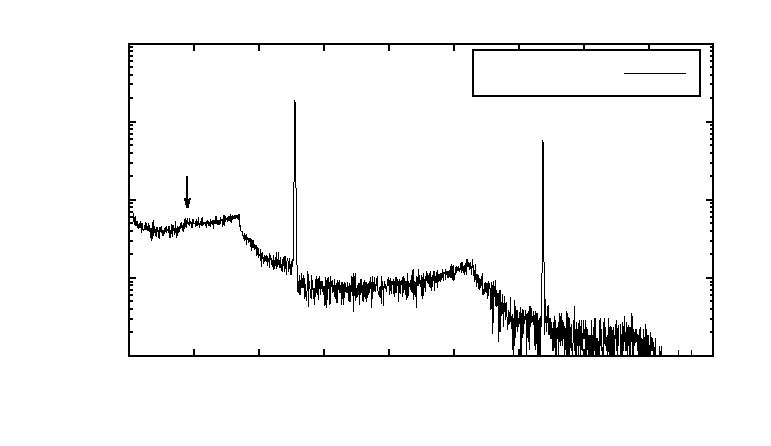
\includegraphics{na-22-spec-back}}%
    \gplfronttext
  \end{picture}%
\endgroup

			\caption{kalibriertes und normiertes $\gamma$-Spektrum der $\prescript{22}{}{\m{Na}}$-Quelle mit abgezogenem normierten und kalibrierten Untergrund}
			\label{fig:na-22-spec-back}
		\end{figure}

		Wie zu erkennen, sind neben dem vorhandenen Rauschen fast nur noch die erwarteten Photopeaks und jeweiligen Comptonkanten zu sehen.
		Durch die Kalibrierung wird allerdings auch der Rückstreupeak der $511\unit{keV}$-Linie sichtbar.

		% Das ist geil.
		% PS: Wir haben geschummelt.
	
	% subsection kalibrierung

	\FloatBarrier
	\subsection{Ein paar andere Spektren}
	\label{ssec:andere spektren}
		
		Nach der gleichen Methode wurden auch die Spektren aller anderen Proben aufgenommen.
		Im Folgenden steht \glqq kalibriert\grqq\ stellvertretend für die Prozedur kalibrieren, normieren und den entsprechenden Untergrund abziehen.
		Für die $\prescript{152}{}{\m{Eu}}$-Quelle und die $\prescript{137}{}{\m{Cs}}$-Quelle ergaben sich demnach die in den Abbildungen \ref{fig:eu-152-spec-back} und \ref{fig:cs-137-spec-back} gezeigten Energieverläufe.
		Beide stimmen sehr gut auf wenige $\unit{keV}$ genau mit den im Anhang \ref{sec:ref-spektren} dargestellten Referenzspektren überein.

		\begin{figure}[htb]
			\centering
			% GNUPLOT: LaTeX picture with Postscript
\begingroup
  \makeatletter
  \providecommand\color[2][]{%
    \GenericError{(gnuplot) \space\space\space\@spaces}{%
      Package color not loaded in conjunction with
      terminal option `colourtext'%
    }{See the gnuplot documentation for explanation.%
    }{Either use 'blacktext' in gnuplot or load the package
      color.sty in LaTeX.}%
    \renewcommand\color[2][]{}%
  }%
  \providecommand\includegraphics[2][]{%
    \GenericError{(gnuplot) \space\space\space\@spaces}{%
      Package graphicx or graphics not loaded%
    }{See the gnuplot documentation for explanation.%
    }{The gnuplot epslatex terminal needs graphicx.sty or graphics.sty.}%
    \renewcommand\includegraphics[2][]{}%
  }%
  \providecommand\rotatebox[2]{#2}%
  \@ifundefined{ifGPcolor}{%
    \newif\ifGPcolor
    \GPcolorfalse
  }{}%
  \@ifundefined{ifGPblacktext}{%
    \newif\ifGPblacktext
    \GPblacktexttrue
  }{}%
  % define a \g@addto@macro without @ in the name:
  \let\gplgaddtomacro\g@addto@macro
  % define empty templates for all commands taking text:
  \gdef\gplbacktext{}%
  \gdef\gplfronttext{}%
  \makeatother
  \ifGPblacktext
    % no textcolor at all
    \def\colorrgb#1{}%
    \def\colorgray#1{}%
  \else
    % gray or color?
    \ifGPcolor
      \def\colorrgb#1{\color[rgb]{#1}}%
      \def\colorgray#1{\color[gray]{#1}}%
      \expandafter\def\csname LTw\endcsname{\color{white}}%
      \expandafter\def\csname LTb\endcsname{\color{black}}%
      \expandafter\def\csname LTa\endcsname{\color{black}}%
      \expandafter\def\csname LT0\endcsname{\color[rgb]{1,0,0}}%
      \expandafter\def\csname LT1\endcsname{\color[rgb]{0,1,0}}%
      \expandafter\def\csname LT2\endcsname{\color[rgb]{0,0,1}}%
      \expandafter\def\csname LT3\endcsname{\color[rgb]{1,0,1}}%
      \expandafter\def\csname LT4\endcsname{\color[rgb]{0,1,1}}%
      \expandafter\def\csname LT5\endcsname{\color[rgb]{1,1,0}}%
      \expandafter\def\csname LT6\endcsname{\color[rgb]{0,0,0}}%
      \expandafter\def\csname LT7\endcsname{\color[rgb]{1,0.3,0}}%
      \expandafter\def\csname LT8\endcsname{\color[rgb]{0.5,0.5,0.5}}%
    \else
      % gray
      \def\colorrgb#1{\color{black}}%
      \def\colorgray#1{\color[gray]{#1}}%
      \expandafter\def\csname LTw\endcsname{\color{white}}%
      \expandafter\def\csname LTb\endcsname{\color{black}}%
      \expandafter\def\csname LTa\endcsname{\color{black}}%
      \expandafter\def\csname LT0\endcsname{\color{black}}%
      \expandafter\def\csname LT1\endcsname{\color{black}}%
      \expandafter\def\csname LT2\endcsname{\color{black}}%
      \expandafter\def\csname LT3\endcsname{\color{black}}%
      \expandafter\def\csname LT4\endcsname{\color{black}}%
      \expandafter\def\csname LT5\endcsname{\color{black}}%
      \expandafter\def\csname LT6\endcsname{\color{black}}%
      \expandafter\def\csname LT7\endcsname{\color{black}}%
      \expandafter\def\csname LT8\endcsname{\color{black}}%
    \fi
  \fi
  \setlength{\unitlength}{0.0500bp}%
  \begin{picture}(7086.00,3968.00)%
    \gplgaddtomacro\gplbacktext{%
      \csname LTb\endcsname%
      \put(814,704){\makebox(0,0)[r]{\strut{}$10^{0}$}}%
      \put(814,1758){\makebox(0,0)[r]{\strut{}$10^{1}$}}%
      \put(814,2812){\makebox(0,0)[r]{\strut{}$10^{2}$}}%
      \put(946,484){\makebox(0,0){\strut{} 0}}%
      \put(1664,484){\makebox(0,0){\strut{} 200}}%
      \put(2382,484){\makebox(0,0){\strut{} 400}}%
      \put(3100,484){\makebox(0,0){\strut{} 600}}%
      \put(3818,484){\makebox(0,0){\strut{} 800}}%
      \put(4535,484){\makebox(0,0){\strut{} 1000}}%
      \put(5253,484){\makebox(0,0){\strut{} 1200}}%
      \put(5971,484){\makebox(0,0){\strut{} 1400}}%
      \put(6689,484){\makebox(0,0){\strut{} 1600}}%
      \put(176,2203){\rotatebox{-270}{\makebox(0,0){\strut{}Intensität}}}%
      \put(3817,154){\makebox(0,0){\strut{}$E \ [\unit{keV}]$}}%
    }%
    \gplgaddtomacro\gplfronttext{%
      \csname LTb\endcsname%
      \put(5702,3420){\makebox(0,0)[r]{\strut{}Messwerte}}%
    }%
    \gplbacktext
    \put(0,0){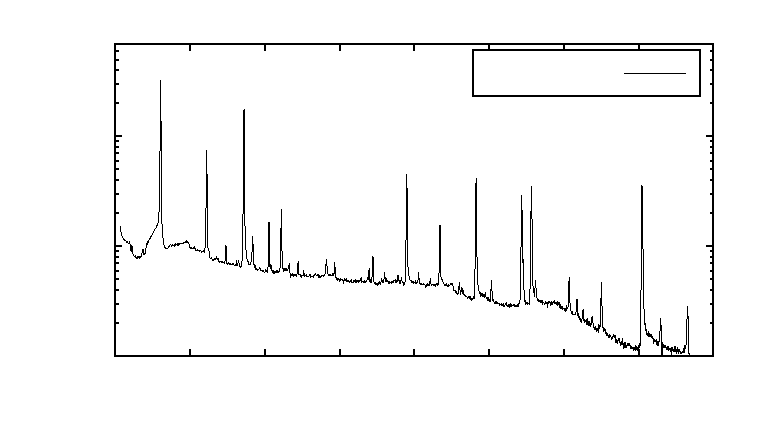
\includegraphics{eu-152-spec-back}}%
    \gplfronttext
  \end{picture}%
\endgroup

			\caption{kalibriertes $\gamma$-Spektrum einer $\prescript{152}{}{\m{Eu}}$-Quelle durch HP-Ge-Detektor aufgenommen in einem Abstand $d=42\unit{cm}$}
			\label{fig:eu-152-spec-back}
		\end{figure}

		Bei $\prescript{137}{}{\m{Cs}}$ sieht man nach Abzug des Untergrundes noch etliche kleinere Peaks mit positiven und negativen Ausschlägen.
		Diese entstehen dadurch, dass zwei verschiedene $\gamma$-Spektren im Allgemeinen nicht dieselben Kalibrierungskoeffizienten $\alpha,\beta$ besitzen.
		Dadurch werden an sich gleiche Energien auf unterschiedliche Kanäle abgebildet.
		Dies resultiert in einer leichten Versetzung der Peaks.
		Somit bleibt nach der Subtraktion ein positiver und negativer Ausschlag.

		\begin{figure}[htb]
			\centering
			% GNUPLOT: LaTeX picture with Postscript
\begingroup
  \makeatletter
  \providecommand\color[2][]{%
    \GenericError{(gnuplot) \space\space\space\@spaces}{%
      Package color not loaded in conjunction with
      terminal option `colourtext'%
    }{See the gnuplot documentation for explanation.%
    }{Either use 'blacktext' in gnuplot or load the package
      color.sty in LaTeX.}%
    \renewcommand\color[2][]{}%
  }%
  \providecommand\includegraphics[2][]{%
    \GenericError{(gnuplot) \space\space\space\@spaces}{%
      Package graphicx or graphics not loaded%
    }{See the gnuplot documentation for explanation.%
    }{The gnuplot epslatex terminal needs graphicx.sty or graphics.sty.}%
    \renewcommand\includegraphics[2][]{}%
  }%
  \providecommand\rotatebox[2]{#2}%
  \@ifundefined{ifGPcolor}{%
    \newif\ifGPcolor
    \GPcolorfalse
  }{}%
  \@ifundefined{ifGPblacktext}{%
    \newif\ifGPblacktext
    \GPblacktexttrue
  }{}%
  % define a \g@addto@macro without @ in the name:
  \let\gplgaddtomacro\g@addto@macro
  % define empty templates for all commands taking text:
  \gdef\gplbacktext{}%
  \gdef\gplfronttext{}%
  \makeatother
  \ifGPblacktext
    % no textcolor at all
    \def\colorrgb#1{}%
    \def\colorgray#1{}%
  \else
    % gray or color?
    \ifGPcolor
      \def\colorrgb#1{\color[rgb]{#1}}%
      \def\colorgray#1{\color[gray]{#1}}%
      \expandafter\def\csname LTw\endcsname{\color{white}}%
      \expandafter\def\csname LTb\endcsname{\color{black}}%
      \expandafter\def\csname LTa\endcsname{\color{black}}%
      \expandafter\def\csname LT0\endcsname{\color[rgb]{1,0,0}}%
      \expandafter\def\csname LT1\endcsname{\color[rgb]{0,1,0}}%
      \expandafter\def\csname LT2\endcsname{\color[rgb]{0,0,1}}%
      \expandafter\def\csname LT3\endcsname{\color[rgb]{1,0,1}}%
      \expandafter\def\csname LT4\endcsname{\color[rgb]{0,1,1}}%
      \expandafter\def\csname LT5\endcsname{\color[rgb]{1,1,0}}%
      \expandafter\def\csname LT6\endcsname{\color[rgb]{0,0,0}}%
      \expandafter\def\csname LT7\endcsname{\color[rgb]{1,0.3,0}}%
      \expandafter\def\csname LT8\endcsname{\color[rgb]{0.5,0.5,0.5}}%
    \else
      % gray
      \def\colorrgb#1{\color{black}}%
      \def\colorgray#1{\color[gray]{#1}}%
      \expandafter\def\csname LTw\endcsname{\color{white}}%
      \expandafter\def\csname LTb\endcsname{\color{black}}%
      \expandafter\def\csname LTa\endcsname{\color{black}}%
      \expandafter\def\csname LT0\endcsname{\color{black}}%
      \expandafter\def\csname LT1\endcsname{\color{black}}%
      \expandafter\def\csname LT2\endcsname{\color{black}}%
      \expandafter\def\csname LT3\endcsname{\color{black}}%
      \expandafter\def\csname LT4\endcsname{\color{black}}%
      \expandafter\def\csname LT5\endcsname{\color{black}}%
      \expandafter\def\csname LT6\endcsname{\color{black}}%
      \expandafter\def\csname LT7\endcsname{\color{black}}%
      \expandafter\def\csname LT8\endcsname{\color{black}}%
    \fi
  \fi
  \setlength{\unitlength}{0.0500bp}%
  \begin{picture}(7086.00,3968.00)%
    \gplgaddtomacro\gplbacktext{%
      \csname LTb\endcsname%
      \put(814,704){\makebox(0,0)[r]{\strut{}$10^{0}$}}%
      \put(814,1704){\makebox(0,0)[r]{\strut{}$10^{1}$}}%
      \put(814,2703){\makebox(0,0)[r]{\strut{}$10^{2}$}}%
      \put(814,3703){\makebox(0,0)[r]{\strut{}$10^{3}$}}%
      \put(946,484){\makebox(0,0){\strut{} 0}}%
      \put(1712,484){\makebox(0,0){\strut{} 100}}%
      \put(2477,484){\makebox(0,0){\strut{} 200}}%
      \put(3243,484){\makebox(0,0){\strut{} 300}}%
      \put(4009,484){\makebox(0,0){\strut{} 400}}%
      \put(4775,484){\makebox(0,0){\strut{} 500}}%
      \put(5540,484){\makebox(0,0){\strut{} 600}}%
      \put(6306,484){\makebox(0,0){\strut{} 700}}%
      \put(176,2203){\rotatebox{-270}{\makebox(0,0){\strut{}Intensität}}}%
      \put(3817,154){\makebox(0,0){\strut{}$E \ [\unit{keV}]$}}%
      \put(1941,2306){\makebox(0,0)[l]{\strut{}\footnotesize Rückstreupeak}}%
    }%
    \gplgaddtomacro\gplfronttext{%
      \csname LTb\endcsname%
      \put(2398,3420){\makebox(0,0)[r]{\strut{}Messwerte}}%
    }%
    \gplbacktext
    \put(0,0){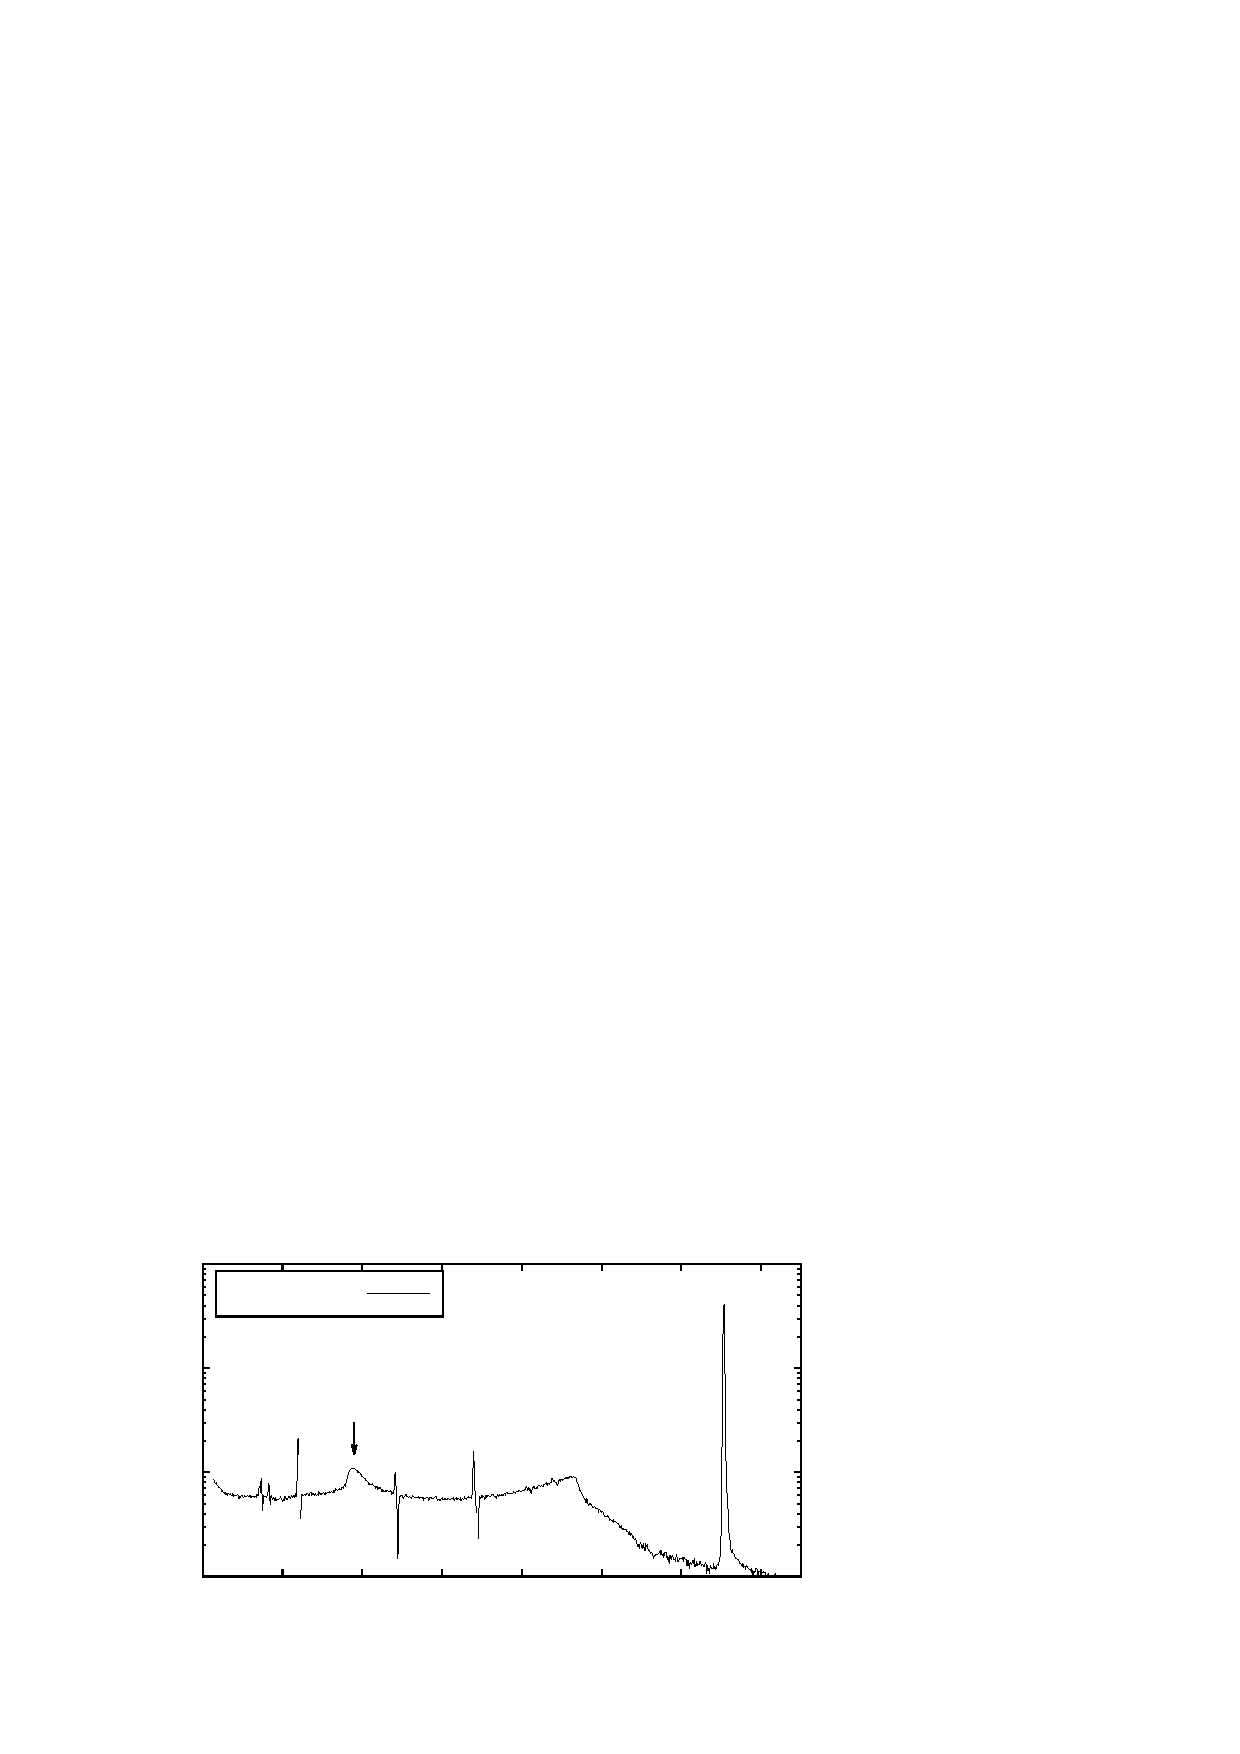
\includegraphics{cs-152-spec-back}}%
    \gplfronttext
  \end{picture}%
\endgroup

			\caption{kalibriertes $\gamma$-Spektrum einer $\prescript{137}{}{\m{Cs}}$-Quelle durch HP-Ge-Detektor aufgenommen in einem Abstand $d=5\unit{cm}$}
			\label{fig:cs-137-spec-back}
		\end{figure}

		Ursachen für die unterschiedlichen Koeffizienten sind zum Beispiel von Messung zu Messung leicht unterschiedliche Temperaturen und damit ein auftretendes thermisches Rauschen beim Detektor, sowie auch Schwankungen in der Messtechnik.

		Aufgrund der einzelnen dominanten $\gamma$-Spektrallinie des $\prescript{137}{}{\m{Cs}}$ bei $660\unit{keV}$ ist nicht nur die zugehörige Comptonkante zu erkennen, sondern auch der stark ausgeprägte Rückstreupeak, wie im Diagramm gekennzeichnet.
		Die Summe der Energien der Comptonkante und des Rückstreupeaks ergibt wieder den entsprechenden Photopeak.
	
	% subsection andere spektren

	% \FloatBarrier
	\subsection{Totzeitkorrektur $\skull$}
	\label{ssec:totzeitkorrektur}

		Während der Messung zeigte sich, dass die gemessenen Counts pro Sekunde (Intensität) $N$ nicht nur von der effektiven Aufnahmezeit $t_\m{live}$ abhängen, sondern auch noch in einer weiteren Beziehung zu der Totzeit$_{\skull}$ $p$ stehen.
		Es wird angenommen, dass die effektiven Counts pro Sekunde $\tilde{N}$ sich aus der folgenden Gleichung für eine gewisse Korrekturfaktorfunktion $K_\skull$ ergeben.
		\[
			\tilde{N} = K_\skull(p) N(p)
		\]
		Um $K_\skull$ zu bestimmen, wurde das Spektrum einer $\prescript{152}{}{\m{Eu}}$-Quelle im Abstand von $30\unit{cm}$ mit dem Spektrum einer $\prescript{137}{}{\m{Cs}}$-Quelle in einem variablen Abstand überlagert.
		Die Veränderung des Abstandes ermöglichte eine Einstellung der Totzeit$_\skull$.
		In Abbildung \ref{fig:totzeit} sind einige ausgewählte Graphen gezeigt.
	
		\begin{figure}[htb]
			\centering
			% GNUPLOT: LaTeX picture with Postscript
\begingroup
  \makeatletter
  \providecommand\color[2][]{%
    \GenericError{(gnuplot) \space\space\space\@spaces}{%
      Package color not loaded in conjunction with
      terminal option `colourtext'%
    }{See the gnuplot documentation for explanation.%
    }{Either use 'blacktext' in gnuplot or load the package
      color.sty in LaTeX.}%
    \renewcommand\color[2][]{}%
  }%
  \providecommand\includegraphics[2][]{%
    \GenericError{(gnuplot) \space\space\space\@spaces}{%
      Package graphicx or graphics not loaded%
    }{See the gnuplot documentation for explanation.%
    }{The gnuplot epslatex terminal needs graphicx.sty or graphics.sty.}%
    \renewcommand\includegraphics[2][]{}%
  }%
  \providecommand\rotatebox[2]{#2}%
  \@ifundefined{ifGPcolor}{%
    \newif\ifGPcolor
    \GPcolorfalse
  }{}%
  \@ifundefined{ifGPblacktext}{%
    \newif\ifGPblacktext
    \GPblacktexttrue
  }{}%
  % define a \g@addto@macro without @ in the name:
  \let\gplgaddtomacro\g@addto@macro
  % define empty templates for all commands taking text:
  \gdef\gplbacktext{}%
  \gdef\gplfronttext{}%
  \makeatother
  \ifGPblacktext
    % no textcolor at all
    \def\colorrgb#1{}%
    \def\colorgray#1{}%
  \else
    % gray or color?
    \ifGPcolor
      \def\colorrgb#1{\color[rgb]{#1}}%
      \def\colorgray#1{\color[gray]{#1}}%
      \expandafter\def\csname LTw\endcsname{\color{white}}%
      \expandafter\def\csname LTb\endcsname{\color{black}}%
      \expandafter\def\csname LTa\endcsname{\color{black}}%
      \expandafter\def\csname LT0\endcsname{\color[rgb]{1,0,0}}%
      \expandafter\def\csname LT1\endcsname{\color[rgb]{0,1,0}}%
      \expandafter\def\csname LT2\endcsname{\color[rgb]{0,0,1}}%
      \expandafter\def\csname LT3\endcsname{\color[rgb]{1,0,1}}%
      \expandafter\def\csname LT4\endcsname{\color[rgb]{0,1,1}}%
      \expandafter\def\csname LT5\endcsname{\color[rgb]{1,1,0}}%
      \expandafter\def\csname LT6\endcsname{\color[rgb]{0,0,0}}%
      \expandafter\def\csname LT7\endcsname{\color[rgb]{1,0.3,0}}%
      \expandafter\def\csname LT8\endcsname{\color[rgb]{0.5,0.5,0.5}}%
    \else
      % gray
      \def\colorrgb#1{\color{black}}%
      \def\colorgray#1{\color[gray]{#1}}%
      \expandafter\def\csname LTw\endcsname{\color{white}}%
      \expandafter\def\csname LTb\endcsname{\color{black}}%
      \expandafter\def\csname LTa\endcsname{\color{black}}%
      \expandafter\def\csname LT0\endcsname{\color{black}}%
      \expandafter\def\csname LT1\endcsname{\color{black}}%
      \expandafter\def\csname LT2\endcsname{\color{black}}%
      \expandafter\def\csname LT3\endcsname{\color{black}}%
      \expandafter\def\csname LT4\endcsname{\color{black}}%
      \expandafter\def\csname LT5\endcsname{\color{black}}%
      \expandafter\def\csname LT6\endcsname{\color{black}}%
      \expandafter\def\csname LT7\endcsname{\color{black}}%
      \expandafter\def\csname LT8\endcsname{\color{black}}%
    \fi
  \fi
  \setlength{\unitlength}{0.0500bp}%
  \begin{picture}(7086.00,3968.00)%
    \gplgaddtomacro\gplbacktext{%
      \csname LTb\endcsname%
      \put(946,704){\makebox(0,0)[r]{\strut{}$10^{-1}$}}%
      \put(946,1401){\makebox(0,0)[r]{\strut{}$10^{0}$}}%
      \put(946,2099){\makebox(0,0)[r]{\strut{}$10^{1}$}}%
      \put(946,2796){\makebox(0,0)[r]{\strut{}$10^{2}$}}%
      \put(946,3493){\makebox(0,0)[r]{\strut{}$10^{3}$}}%
      \put(1078,484){\makebox(0,0){\strut{} 0}}%
      \put(1779,484){\makebox(0,0){\strut{} 100}}%
      \put(2481,484){\makebox(0,0){\strut{} 200}}%
      \put(3182,484){\makebox(0,0){\strut{} 300}}%
      \put(3884,484){\makebox(0,0){\strut{} 400}}%
      \put(4585,484){\makebox(0,0){\strut{} 500}}%
      \put(5286,484){\makebox(0,0){\strut{} 600}}%
      \put(5988,484){\makebox(0,0){\strut{} 700}}%
      \put(6689,484){\makebox(0,0){\strut{} 800}}%
      \put(176,2203){\rotatebox{-270}{\makebox(0,0){\strut{}Intensität}}}%
      \put(3883,154){\makebox(0,0){\strut{}Kanal}}%
    }%
    \gplgaddtomacro\gplfronttext{%
      \csname LTb\endcsname%
      \put(2002,3420){\makebox(0,0)[r]{\strut{}$50\unit{cm}$}}%
      \csname LTb\endcsname%
      \put(2002,3200){\makebox(0,0)[r]{\strut{}$15\unit{cm}$}}%
      \csname LTb\endcsname%
      \put(2002,2980){\makebox(0,0)[r]{\strut{}$5\unit{cm}$}}%
      \csname LTb\endcsname%
      \put(2002,2760){\makebox(0,0)[r]{\strut{}$0\unit{cm}$}}%
    }%
    \gplbacktext
    \put(0,0){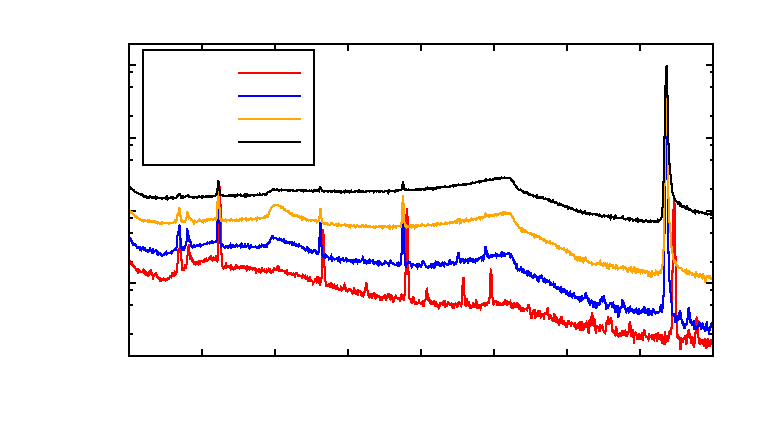
\includegraphics{totzeit}}%
    \gplfronttext
  \end{picture}%
\endgroup

			\caption{Ausschnitt der $\gamma$-Spektren einer $\prescript{152}{}{\m{Eu}}$-Quelle im Abstand $d_\m{Eu}=30\unit{cm}$ überlagert mit denen einer $\prescript{137}{}{\m{Cs}}$-Quelle in variablen Abständen aufgenommen durch den HP-Ge-Detektor}
			\label{fig:totzeit}
		\end{figure}

		Anhand der $344\unit{keV}$-Linie des Eu wurde nun die Abhängigkeit der Intensität $N$ oder auch Counts pro Sekunde von der Totzeit$_\skull$ $p$ untersucht.
		In Abbildung \ref{fig:totzeit-k} sind die Messwerte durch eine lineare Funktion sehr gut approximiert.
		Man kann also annehmen, dass für gewisse Konstanten $a,b$ folgender Zusammenhang besteht.
		\[
			N(p) = ap+b \quad \implies \quad K_\skull(p) = \frac{b}{ap+b}
		\]

		\begin{figure}[htb]
			\centering
			% GNUPLOT: LaTeX picture with Postscript
\begingroup
  \makeatletter
  \providecommand\color[2][]{%
    \GenericError{(gnuplot) \space\space\space\@spaces}{%
      Package color not loaded in conjunction with
      terminal option `colourtext'%
    }{See the gnuplot documentation for explanation.%
    }{Either use 'blacktext' in gnuplot or load the package
      color.sty in LaTeX.}%
    \renewcommand\color[2][]{}%
  }%
  \providecommand\includegraphics[2][]{%
    \GenericError{(gnuplot) \space\space\space\@spaces}{%
      Package graphicx or graphics not loaded%
    }{See the gnuplot documentation for explanation.%
    }{The gnuplot epslatex terminal needs graphicx.sty or graphics.sty.}%
    \renewcommand\includegraphics[2][]{}%
  }%
  \providecommand\rotatebox[2]{#2}%
  \@ifundefined{ifGPcolor}{%
    \newif\ifGPcolor
    \GPcolorfalse
  }{}%
  \@ifundefined{ifGPblacktext}{%
    \newif\ifGPblacktext
    \GPblacktexttrue
  }{}%
  % define a \g@addto@macro without @ in the name:
  \let\gplgaddtomacro\g@addto@macro
  % define empty templates for all commands taking text:
  \gdef\gplbacktext{}%
  \gdef\gplfronttext{}%
  \makeatother
  \ifGPblacktext
    % no textcolor at all
    \def\colorrgb#1{}%
    \def\colorgray#1{}%
  \else
    % gray or color?
    \ifGPcolor
      \def\colorrgb#1{\color[rgb]{#1}}%
      \def\colorgray#1{\color[gray]{#1}}%
      \expandafter\def\csname LTw\endcsname{\color{white}}%
      \expandafter\def\csname LTb\endcsname{\color{black}}%
      \expandafter\def\csname LTa\endcsname{\color{black}}%
      \expandafter\def\csname LT0\endcsname{\color[rgb]{1,0,0}}%
      \expandafter\def\csname LT1\endcsname{\color[rgb]{0,1,0}}%
      \expandafter\def\csname LT2\endcsname{\color[rgb]{0,0,1}}%
      \expandafter\def\csname LT3\endcsname{\color[rgb]{1,0,1}}%
      \expandafter\def\csname LT4\endcsname{\color[rgb]{0,1,1}}%
      \expandafter\def\csname LT5\endcsname{\color[rgb]{1,1,0}}%
      \expandafter\def\csname LT6\endcsname{\color[rgb]{0,0,0}}%
      \expandafter\def\csname LT7\endcsname{\color[rgb]{1,0.3,0}}%
      \expandafter\def\csname LT8\endcsname{\color[rgb]{0.5,0.5,0.5}}%
    \else
      % gray
      \def\colorrgb#1{\color{black}}%
      \def\colorgray#1{\color[gray]{#1}}%
      \expandafter\def\csname LTw\endcsname{\color{white}}%
      \expandafter\def\csname LTb\endcsname{\color{black}}%
      \expandafter\def\csname LTa\endcsname{\color{black}}%
      \expandafter\def\csname LT0\endcsname{\color{black}}%
      \expandafter\def\csname LT1\endcsname{\color{black}}%
      \expandafter\def\csname LT2\endcsname{\color{black}}%
      \expandafter\def\csname LT3\endcsname{\color{black}}%
      \expandafter\def\csname LT4\endcsname{\color{black}}%
      \expandafter\def\csname LT5\endcsname{\color{black}}%
      \expandafter\def\csname LT6\endcsname{\color{black}}%
      \expandafter\def\csname LT7\endcsname{\color{black}}%
      \expandafter\def\csname LT8\endcsname{\color{black}}%
    \fi
  \fi
  \setlength{\unitlength}{0.0500bp}%
  \begin{picture}(7086.00,3968.00)%
    \gplgaddtomacro\gplbacktext{%
      \csname LTb\endcsname%
      \put(814,704){\makebox(0,0)[r]{\strut{} 10}}%
      \put(814,1454){\makebox(0,0)[r]{\strut{} 15}}%
      \put(814,2204){\makebox(0,0)[r]{\strut{} 20}}%
      \put(814,2953){\makebox(0,0)[r]{\strut{} 25}}%
      \put(814,3703){\makebox(0,0)[r]{\strut{} 30}}%
      \put(946,484){\makebox(0,0){\strut{} 0}}%
      \put(1830,484){\makebox(0,0){\strut{} 10}}%
      \put(2713,484){\makebox(0,0){\strut{} 20}}%
      \put(3597,484){\makebox(0,0){\strut{} 30}}%
      \put(4480,484){\makebox(0,0){\strut{} 40}}%
      \put(5364,484){\makebox(0,0){\strut{} 50}}%
      \put(6247,484){\makebox(0,0){\strut{} 60}}%
      \put(176,2203){\rotatebox{-270}{\makebox(0,0){\strut{}Intensität}}}%
      \put(3817,154){\makebox(0,0){\strut{}relative Totzeit$_\skull \ [\unit{\%}]$}}%
    }%
    \gplgaddtomacro\gplfronttext{%
      \csname LTb\endcsname%
      \put(2926,3420){\makebox(0,0)[r]{\strut{}\footnotesize Messwerte}}%
      \csname LTb\endcsname%
      \put(2926,3200){\makebox(0,0)[r]{\strut{}\footnotesize $f(x) = ax+b$}}%
    }%
    \gplbacktext
    \put(0,0){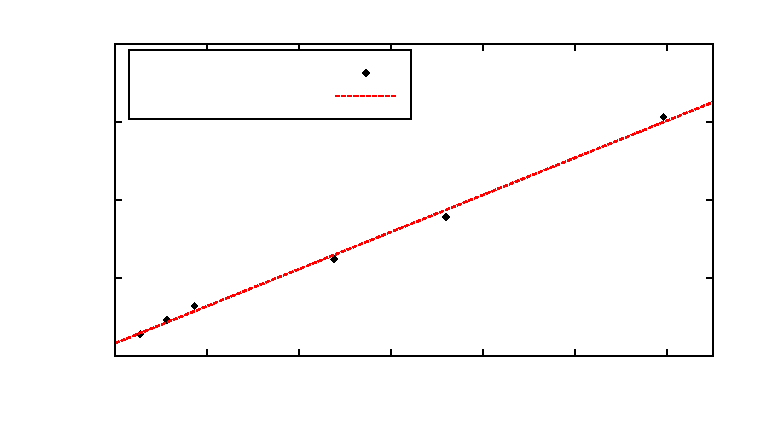
\includegraphics{totzeit-k}}%
    \gplfronttext
  \end{picture}%
\endgroup

			\caption{Intensitäten des $344\unit{keV}$-Photopeaks von $\prescript{152}{}{\m{Eu}}$ in Abhängigkeit der relativen Totzeit$_\skull$ mit linearem Fit $f$ \\ Parameter: $a=0.23757\unit{\inv{s}}$, $b=10.8203\unit{\inv{s}}$}
			\label{fig:totzeit-k}
		\end{figure}
		
		Aus dem Diagramm ergeben sich für die Konstanten
		\[
			a=0.23757\unit{\inv{s}},\qquad b=10.8203\unit{\inv{s}}
		\]
		Betrachtet man nun charakteristische $\gamma$-Linie des Cs, so können die gemessenen Intensitäten nun mithilfe der Korrekturfunktion auf die erwartete $r^{-2}$-Gesetzmäßigkeit untersucht werden.
		Das Ergebnis ist in Abbildung \ref{fig:abstand} zu sehen.
		Dieses deckt sich mit den in den Grundlagen angegebenen Erwartungen.

		\begin{figure}[htb]
			\centering
			% GNUPLOT: LaTeX picture with Postscript
\begingroup
  \makeatletter
  \providecommand\color[2][]{%
    \GenericError{(gnuplot) \space\space\space\@spaces}{%
      Package color not loaded in conjunction with
      terminal option `colourtext'%
    }{See the gnuplot documentation for explanation.%
    }{Either use 'blacktext' in gnuplot or load the package
      color.sty in LaTeX.}%
    \renewcommand\color[2][]{}%
  }%
  \providecommand\includegraphics[2][]{%
    \GenericError{(gnuplot) \space\space\space\@spaces}{%
      Package graphicx or graphics not loaded%
    }{See the gnuplot documentation for explanation.%
    }{The gnuplot epslatex terminal needs graphicx.sty or graphics.sty.}%
    \renewcommand\includegraphics[2][]{}%
  }%
  \providecommand\rotatebox[2]{#2}%
  \@ifundefined{ifGPcolor}{%
    \newif\ifGPcolor
    \GPcolorfalse
  }{}%
  \@ifundefined{ifGPblacktext}{%
    \newif\ifGPblacktext
    \GPblacktexttrue
  }{}%
  % define a \g@addto@macro without @ in the name:
  \let\gplgaddtomacro\g@addto@macro
  % define empty templates for all commands taking text:
  \gdef\gplbacktext{}%
  \gdef\gplfronttext{}%
  \makeatother
  \ifGPblacktext
    % no textcolor at all
    \def\colorrgb#1{}%
    \def\colorgray#1{}%
  \else
    % gray or color?
    \ifGPcolor
      \def\colorrgb#1{\color[rgb]{#1}}%
      \def\colorgray#1{\color[gray]{#1}}%
      \expandafter\def\csname LTw\endcsname{\color{white}}%
      \expandafter\def\csname LTb\endcsname{\color{black}}%
      \expandafter\def\csname LTa\endcsname{\color{black}}%
      \expandafter\def\csname LT0\endcsname{\color[rgb]{1,0,0}}%
      \expandafter\def\csname LT1\endcsname{\color[rgb]{0,1,0}}%
      \expandafter\def\csname LT2\endcsname{\color[rgb]{0,0,1}}%
      \expandafter\def\csname LT3\endcsname{\color[rgb]{1,0,1}}%
      \expandafter\def\csname LT4\endcsname{\color[rgb]{0,1,1}}%
      \expandafter\def\csname LT5\endcsname{\color[rgb]{1,1,0}}%
      \expandafter\def\csname LT6\endcsname{\color[rgb]{0,0,0}}%
      \expandafter\def\csname LT7\endcsname{\color[rgb]{1,0.3,0}}%
      \expandafter\def\csname LT8\endcsname{\color[rgb]{0.5,0.5,0.5}}%
    \else
      % gray
      \def\colorrgb#1{\color{black}}%
      \def\colorgray#1{\color[gray]{#1}}%
      \expandafter\def\csname LTw\endcsname{\color{white}}%
      \expandafter\def\csname LTb\endcsname{\color{black}}%
      \expandafter\def\csname LTa\endcsname{\color{black}}%
      \expandafter\def\csname LT0\endcsname{\color{black}}%
      \expandafter\def\csname LT1\endcsname{\color{black}}%
      \expandafter\def\csname LT2\endcsname{\color{black}}%
      \expandafter\def\csname LT3\endcsname{\color{black}}%
      \expandafter\def\csname LT4\endcsname{\color{black}}%
      \expandafter\def\csname LT5\endcsname{\color{black}}%
      \expandafter\def\csname LT6\endcsname{\color{black}}%
      \expandafter\def\csname LT7\endcsname{\color{black}}%
      \expandafter\def\csname LT8\endcsname{\color{black}}%
    \fi
  \fi
  \setlength{\unitlength}{0.0500bp}%
  \begin{picture}(7086.00,3968.00)%
    \gplgaddtomacro\gplbacktext{%
      \csname LTb\endcsname%
      \put(946,704){\makebox(0,0)[r]{\strut{} 0}}%
      \put(946,1304){\makebox(0,0)[r]{\strut{} 100}}%
      \put(946,1904){\makebox(0,0)[r]{\strut{} 200}}%
      \put(946,2503){\makebox(0,0)[r]{\strut{} 300}}%
      \put(946,3103){\makebox(0,0)[r]{\strut{} 400}}%
      \put(946,3703){\makebox(0,0)[r]{\strut{} 500}}%
      \put(1078,484){\makebox(0,0){\strut{} 0}}%
      \put(2200,484){\makebox(0,0){\strut{} 5}}%
      \put(3322,484){\makebox(0,0){\strut{} 10}}%
      \put(4445,484){\makebox(0,0){\strut{} 15}}%
      \put(5567,484){\makebox(0,0){\strut{} 20}}%
      \put(6689,484){\makebox(0,0){\strut{} 25}}%
      \put(176,2203){\rotatebox{-270}{\makebox(0,0){\strut{}Intensität}}}%
      \put(3883,154){\makebox(0,0){\strut{}Abstand $d \ [\unit{cm}]$}}%
    }%
    \gplgaddtomacro\gplfronttext{%
      \csname LTb\endcsname%
      \put(5702,3420){\makebox(0,0)[r]{\strut{}\footnotesize Messwerte}}%
      \csname LTb\endcsname%
      \put(5702,3200){\makebox(0,0)[r]{\strut{}\footnotesize Fit}}%
    }%
    \gplbacktext
    \put(0,0){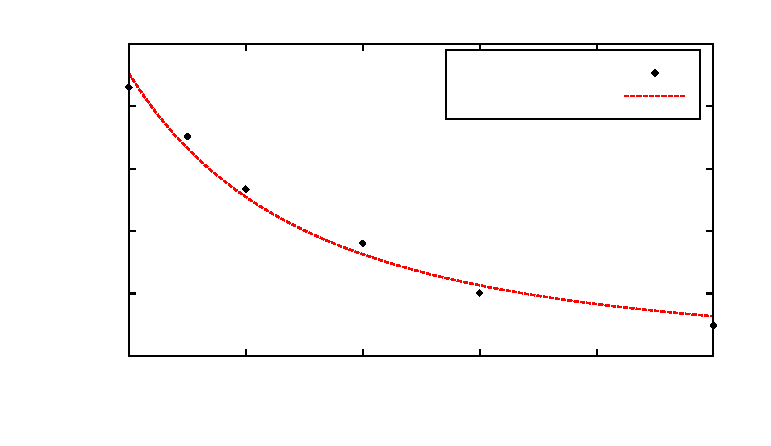
\includegraphics{abstand}}%
    \gplfronttext
  \end{picture}%
\endgroup

			\caption{Abhängigkeit der korrigierten Intensität des $660\unit{keV}$-Peaks von Cs vom Probenabstand $d$}
			\label{fig:abstand}
		\end{figure}
	
	% subsection totzeitkorrektur

	\FloatBarrier
	\subsection{Vergleich der Detektoren}
	\label{ssec:vergleich}

		Im Versuch standen neben dem HP-Ge-Detektor noch zwei Szintillationsdetektoren zur Verfügung.
		Um Vergleiche zwischen deren Aufnahmen anstellen zu können, wurde von jedem ein Spektrum der gleichen $\prescript{22}{}{\m{Na}}$-Quelle aufgenommen.
		Die entstanden Spektren wurden leicht angepasst und sind in Graph \ref{fig:detektoren} dargestellt.
	
		\begin{figure}[htb]
			\centering
			% GNUPLOT: LaTeX picture with Postscript
\begingroup
  \makeatletter
  \providecommand\color[2][]{%
    \GenericError{(gnuplot) \space\space\space\@spaces}{%
      Package color not loaded in conjunction with
      terminal option `colourtext'%
    }{See the gnuplot documentation for explanation.%
    }{Either use 'blacktext' in gnuplot or load the package
      color.sty in LaTeX.}%
    \renewcommand\color[2][]{}%
  }%
  \providecommand\includegraphics[2][]{%
    \GenericError{(gnuplot) \space\space\space\@spaces}{%
      Package graphicx or graphics not loaded%
    }{See the gnuplot documentation for explanation.%
    }{The gnuplot epslatex terminal needs graphicx.sty or graphics.sty.}%
    \renewcommand\includegraphics[2][]{}%
  }%
  \providecommand\rotatebox[2]{#2}%
  \@ifundefined{ifGPcolor}{%
    \newif\ifGPcolor
    \GPcolorfalse
  }{}%
  \@ifundefined{ifGPblacktext}{%
    \newif\ifGPblacktext
    \GPblacktexttrue
  }{}%
  % define a \g@addto@macro without @ in the name:
  \let\gplgaddtomacro\g@addto@macro
  % define empty templates for all commands taking text:
  \gdef\gplbacktext{}%
  \gdef\gplfronttext{}%
  \makeatother
  \ifGPblacktext
    % no textcolor at all
    \def\colorrgb#1{}%
    \def\colorgray#1{}%
  \else
    % gray or color?
    \ifGPcolor
      \def\colorrgb#1{\color[rgb]{#1}}%
      \def\colorgray#1{\color[gray]{#1}}%
      \expandafter\def\csname LTw\endcsname{\color{white}}%
      \expandafter\def\csname LTb\endcsname{\color{black}}%
      \expandafter\def\csname LTa\endcsname{\color{black}}%
      \expandafter\def\csname LT0\endcsname{\color[rgb]{1,0,0}}%
      \expandafter\def\csname LT1\endcsname{\color[rgb]{0,1,0}}%
      \expandafter\def\csname LT2\endcsname{\color[rgb]{0,0,1}}%
      \expandafter\def\csname LT3\endcsname{\color[rgb]{1,0,1}}%
      \expandafter\def\csname LT4\endcsname{\color[rgb]{0,1,1}}%
      \expandafter\def\csname LT5\endcsname{\color[rgb]{1,1,0}}%
      \expandafter\def\csname LT6\endcsname{\color[rgb]{0,0,0}}%
      \expandafter\def\csname LT7\endcsname{\color[rgb]{1,0.3,0}}%
      \expandafter\def\csname LT8\endcsname{\color[rgb]{0.5,0.5,0.5}}%
    \else
      % gray
      \def\colorrgb#1{\color{black}}%
      \def\colorgray#1{\color[gray]{#1}}%
      \expandafter\def\csname LTw\endcsname{\color{white}}%
      \expandafter\def\csname LTb\endcsname{\color{black}}%
      \expandafter\def\csname LTa\endcsname{\color{black}}%
      \expandafter\def\csname LT0\endcsname{\color{black}}%
      \expandafter\def\csname LT1\endcsname{\color{black}}%
      \expandafter\def\csname LT2\endcsname{\color{black}}%
      \expandafter\def\csname LT3\endcsname{\color{black}}%
      \expandafter\def\csname LT4\endcsname{\color{black}}%
      \expandafter\def\csname LT5\endcsname{\color{black}}%
      \expandafter\def\csname LT6\endcsname{\color{black}}%
      \expandafter\def\csname LT7\endcsname{\color{black}}%
      \expandafter\def\csname LT8\endcsname{\color{black}}%
    \fi
  \fi
  \setlength{\unitlength}{0.0500bp}%
  \begin{picture}(7086.00,3968.00)%
    \gplgaddtomacro\gplbacktext{%
      \csname LTb\endcsname%
      \put(946,704){\makebox(0,0)[r]{\strut{}$10^{-2}$}}%
      \put(946,1374){\makebox(0,0)[r]{\strut{}$10^{-1}$}}%
      \put(946,2044){\makebox(0,0)[r]{\strut{}$10^{0}$}}%
      \put(946,2714){\makebox(0,0)[r]{\strut{}$10^{1}$}}%
      \put(946,3383){\makebox(0,0)[r]{\strut{}$10^{2}$}}%
      \put(1078,484){\makebox(0,0){\strut{} 200}}%
      \put(1779,484){\makebox(0,0){\strut{} 400}}%
      \put(2481,484){\makebox(0,0){\strut{} 600}}%
      \put(3182,484){\makebox(0,0){\strut{} 800}}%
      \put(3884,484){\makebox(0,0){\strut{} 1000}}%
      \put(4585,484){\makebox(0,0){\strut{} 1200}}%
      \put(5286,484){\makebox(0,0){\strut{} 1400}}%
      \put(5988,484){\makebox(0,0){\strut{} 1600}}%
      \put(6689,484){\makebox(0,0){\strut{} 1800}}%
      \put(176,2203){\rotatebox{-270}{\makebox(0,0){\strut{}Intensität}}}%
      \put(3883,154){\makebox(0,0){\strut{}$E \ [\unit{keV}]$}}%
    }%
    \gplgaddtomacro\gplfronttext{%
      \csname LTb\endcsname%
      \put(5702,3420){\makebox(0,0)[r]{\strut{}\footnotesize HP-Ge-Detektor}}%
      \csname LTb\endcsname%
      \put(5702,3200){\makebox(0,0)[r]{\strut{}\footnotesize NaI(Tl)-Detektor}}%
      \csname LTb\endcsname%
      \put(5702,2980){\makebox(0,0)[r]{\strut{}\footnotesize Plastik}}%
    }%
    \gplbacktext
    \put(0,0){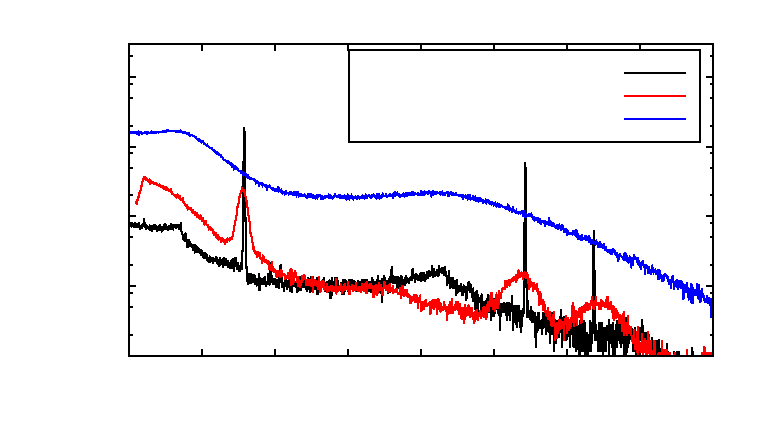
\includegraphics{detektoren}}%
    \gplfronttext
  \end{picture}%
\endgroup

			\caption{angepasstes $\gamma$-Spektrum der $\prescript{22}{}{\m{Na}}$-Quelle mit $d=5\unit{cm}$ aufgenommen durch verschiedene Detektortypen}
			\label{fig:detektoren}
		\end{figure}

		Eine Gegenüberstellung zeigt sogleich, dass die Vollabsorptionspeaks beim Plastik-Detektor fehlen, während sie beim NaI-Detektor zwar an der richtigen Stelle, aber mit wesentlich geringerer Auflösung auftreten.
		Das Fehlen bei Plastik ist darauf zurück zu führen, dass für den Photoeffekt wie in den Grundlagen erklärt sehr stark gebundene Elektronen und somit hohe Kernladungszahlen $Z$ von Nöten sind.
		Da Kunststoff jedoch meist aus organischen Verbindungen mit Kohlenstoff, Wasserstoff, Sauerstoff und Stickstoff besteht, fehlen hier die Elemente mit hohem $Z$, weshalb in diesem Material bevorzugt Compton-Streuung auftritt.
		Die entsprechenden Comptonkannten sind hingegen bei beiden Szintillatortypen gut zu erkennen.
		Die geringere Auflösung des NaI-Detektors lässt sich mit der niedrigeren Signalzahl $N_S$ erklären, siehe hierzu Abschnitt \ref{ssec:aufloesung}.
	
	% subsection vergleich

	\FloatBarrier
	\subsection{Auflösungsvermögen}
	\label{ssec:aufloesung}
	
		Um das Auflösungsvermögen des HP-Ge-Detektors zu untersuchen wurde zunächst der Ausschnitt der $511 \unit{keV} $-Linie vergrößert; das Ergebnis ist in Abbildung \ref{fig:gauss} zu sehen.

		\begin{figure}[htb]
			\centering
			% GNUPLOT: LaTeX picture with Postscript
\begingroup
  \makeatletter
  \providecommand\color[2][]{%
    \GenericError{(gnuplot) \space\space\space\@spaces}{%
      Package color not loaded in conjunction with
      terminal option `colourtext'%
    }{See the gnuplot documentation for explanation.%
    }{Either use 'blacktext' in gnuplot or load the package
      color.sty in LaTeX.}%
    \renewcommand\color[2][]{}%
  }%
  \providecommand\includegraphics[2][]{%
    \GenericError{(gnuplot) \space\space\space\@spaces}{%
      Package graphicx or graphics not loaded%
    }{See the gnuplot documentation for explanation.%
    }{The gnuplot epslatex terminal needs graphicx.sty or graphics.sty.}%
    \renewcommand\includegraphics[2][]{}%
  }%
  \providecommand\rotatebox[2]{#2}%
  \@ifundefined{ifGPcolor}{%
    \newif\ifGPcolor
    \GPcolorfalse
  }{}%
  \@ifundefined{ifGPblacktext}{%
    \newif\ifGPblacktext
    \GPblacktexttrue
  }{}%
  % define a \g@addto@macro without @ in the name:
  \let\gplgaddtomacro\g@addto@macro
  % define empty templates for all commands taking text:
  \gdef\gplbacktext{}%
  \gdef\gplfronttext{}%
  \makeatother
  \ifGPblacktext
    % no textcolor at all
    \def\colorrgb#1{}%
    \def\colorgray#1{}%
  \else
    % gray or color?
    \ifGPcolor
      \def\colorrgb#1{\color[rgb]{#1}}%
      \def\colorgray#1{\color[gray]{#1}}%
      \expandafter\def\csname LTw\endcsname{\color{white}}%
      \expandafter\def\csname LTb\endcsname{\color{black}}%
      \expandafter\def\csname LTa\endcsname{\color{black}}%
      \expandafter\def\csname LT0\endcsname{\color[rgb]{1,0,0}}%
      \expandafter\def\csname LT1\endcsname{\color[rgb]{0,1,0}}%
      \expandafter\def\csname LT2\endcsname{\color[rgb]{0,0,1}}%
      \expandafter\def\csname LT3\endcsname{\color[rgb]{1,0,1}}%
      \expandafter\def\csname LT4\endcsname{\color[rgb]{0,1,1}}%
      \expandafter\def\csname LT5\endcsname{\color[rgb]{1,1,0}}%
      \expandafter\def\csname LT6\endcsname{\color[rgb]{0,0,0}}%
      \expandafter\def\csname LT7\endcsname{\color[rgb]{1,0.3,0}}%
      \expandafter\def\csname LT8\endcsname{\color[rgb]{0.5,0.5,0.5}}%
    \else
      % gray
      \def\colorrgb#1{\color{black}}%
      \def\colorgray#1{\color[gray]{#1}}%
      \expandafter\def\csname LTw\endcsname{\color{white}}%
      \expandafter\def\csname LTb\endcsname{\color{black}}%
      \expandafter\def\csname LTa\endcsname{\color{black}}%
      \expandafter\def\csname LT0\endcsname{\color{black}}%
      \expandafter\def\csname LT1\endcsname{\color{black}}%
      \expandafter\def\csname LT2\endcsname{\color{black}}%
      \expandafter\def\csname LT3\endcsname{\color{black}}%
      \expandafter\def\csname LT4\endcsname{\color{black}}%
      \expandafter\def\csname LT5\endcsname{\color{black}}%
      \expandafter\def\csname LT6\endcsname{\color{black}}%
      \expandafter\def\csname LT7\endcsname{\color{black}}%
      \expandafter\def\csname LT8\endcsname{\color{black}}%
    \fi
  \fi
  \setlength{\unitlength}{0.0500bp}%
  \begin{picture}(7086.00,3968.00)%
    \gplgaddtomacro\gplbacktext{%
      \csname LTb\endcsname%
      \put(814,704){\makebox(0,0)[r]{\strut{} 0}}%
      \put(814,1004){\makebox(0,0)[r]{\strut{} 2}}%
      \put(814,1304){\makebox(0,0)[r]{\strut{} 4}}%
      \put(814,1604){\makebox(0,0)[r]{\strut{} 6}}%
      \put(814,1904){\makebox(0,0)[r]{\strut{} 8}}%
      \put(814,2204){\makebox(0,0)[r]{\strut{} 10}}%
      \put(814,2503){\makebox(0,0)[r]{\strut{} 12}}%
      \put(814,2803){\makebox(0,0)[r]{\strut{} 14}}%
      \put(814,3103){\makebox(0,0)[r]{\strut{} 16}}%
      \put(814,3403){\makebox(0,0)[r]{\strut{} 18}}%
      \put(814,3703){\makebox(0,0)[r]{\strut{} 20}}%
      \put(1329,484){\makebox(0,0){\strut{} 506}}%
      \put(2095,484){\makebox(0,0){\strut{} 508}}%
      \put(2860,484){\makebox(0,0){\strut{} 510}}%
      \put(3626,484){\makebox(0,0){\strut{} 512}}%
      \put(4392,484){\makebox(0,0){\strut{} 514}}%
      \put(5158,484){\makebox(0,0){\strut{} 516}}%
      \put(5923,484){\makebox(0,0){\strut{} 518}}%
      \put(6689,484){\makebox(0,0){\strut{} 520}}%
      \put(176,2203){\rotatebox{-270}{\makebox(0,0){\strut{}Intensität}}}%
      \put(3817,154){\makebox(0,0){\strut{}$E \ [\unit{keV}]$}}%
    }%
    \gplgaddtomacro\gplfronttext{%
      \csname LTb\endcsname%
      \put(5702,3420){\makebox(0,0)[r]{\strut{}\footnotesize Gauß-Fit}}%
      \csname LTb\endcsname%
      \put(5702,3200){\makebox(0,0)[r]{\strut{}\footnotesize Messwerte}}%
    }%
    \gplbacktext
    \put(0,0){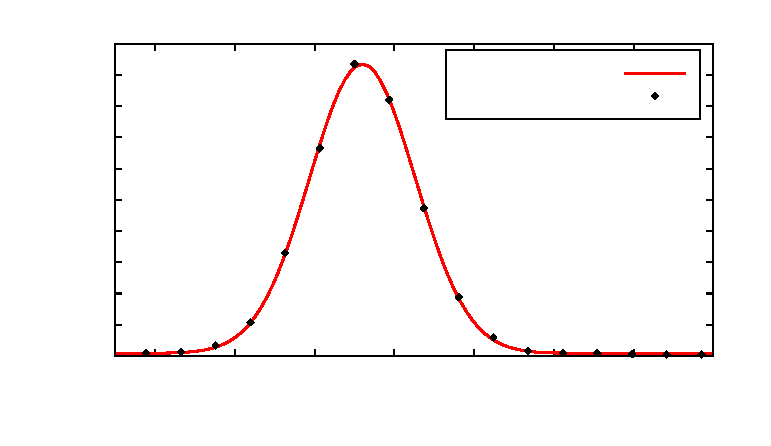
\includegraphics{gauss}}%
    \gplfronttext
  \end{picture}%
\endgroup

			\caption{Ausschnitt des $511\unit{keV}$-Photopeaks aus dem kalibrierten $\gamma$-Spektrum der $\prescript{22}{}{\m{Na}}$-Quelle mit $d=0\unit{cm}$ und einer gefitteten Gauß-Normalverteilung}
			\label{fig:gauss}
		\end{figure}

		Die Messpunkte wurden mit Hilfe eines Gauß-Fits der folgenden Form angepasst. 
		\[ f(x) = C \exp\curvb{- \frac{1}{2} \frac{(x - \mu)^2}{\sigma ^2}} + K \]
		Hierbei bezeichnen $C,\mu,\sigma,K$ die Variablen Parameter.
		Für die Varianz $\sigma$ ergab sich
		
		\[ \sigma = 1.33 \unit{keV}\]

		Damit liegt $\sigma$ sehr weit oberhalb der natürlichen Linienbreite.
		Die Verbreiterung geschieht durch statistische Prozesse bei der Energieabgabe des Primärelektrons.
		Für die Energieauflösung $A$ ergibt sich
		\[
		 	A = \frac{E_\gamma}{\Delta E} = \frac{E_\gamma}{\sigma} = 
		 	\frac{N_\m{LT}}{\sigma_\m{LT}} 
		 \] 
		Hierbei ist $N_\m{LT}$ die Zahl der durch das Primärelektron erzeugten Ladungsträger, also gilt $N_{\m{LT}} \sim E_\gamma $.
		Bei Annahme einer Poissonverteilung wäre $\sigma ^2 = N_{\m{LT}} $.
		Im Allgemeinen ist die Varianz jedoch kleiner, was durch die Einführung des Fano-Faktors $F < 1$ berücksichtigt wird.
		Für Ge-Detektoren beträgt dieser etwa $F = 0.1$
		\[
			\implies \quad A_\m{Ge} = \frac{511 \unit{keV} }{1.33\unit{keV} } \approx 384
		\]
		Hätte man jetzt auch nur die leiseste Ahnung, welcher Kanal mit welcher ursprünglichen Ladungträgeranzahl verknüpft wäre, man könnte glatt die Energie zur Erzeugung eines Elektron-Loch-Paares aufschreiben.
		% \[
		% 	\implies N_\m{LT} = \sigma^2 / F \approx 01234071236508276
		% \]
		% Aus den durch das Primärelektron ausgelösten Elektron-Loch-Paaren und seiner Energie lässt sich nun die notwendige Arbeit $W_{\m{Paar} } $ zu Erzeugung eines Paares berechnen:
		% \[
		% 	W_{\m{Paar}} = \frac{E_\gamma}{N_\m{LT}}
		% \]

		Für den NaI-Detektor ergab sich analog ein $\sigma$ von
		\[
			\sigma  = 10.99 \unit{keV} \quad \implies \quad A = \frac{511}{10.99} \approx 46.5
		\]
		Die kleinere Auflösung liegt an der wesentlich kleineren Anzahl an Photonen die vom Primärelekton ausgelöst werden und den Photomultiplier auch wirklich erreichen.

	% subsection aufloesung

	\FloatBarrier
	\subsection{Nachweiswahrscheinlichkeit}
	\label{ssec:Nachweiswahrscheinlichkeit}
	
		Aus der Versuchsvorbereitung ist bekannt
		\[
			\tilde{N} = \varepsilon \alpha A
		\]
		Dabei ist $\alpha$ die Emissionswahrscheinlichkeit eines $\gamma$-Quants durch einen Zerfall, $\varepsilon$ die Nachweiswahrscheinlichkeit und $A$ die Aktivität der Probe.
		$\varepsilon$ wird anhand des $\prescript{22}{}{\m{Na}}$-Spektrums berechnet.
		Für den $511\unit{keV}$-Peak und den $1275\unit{keV}$-Peak ergeben sich durch Rechnung und Datenblätter
		\[
			\tilde{N}_{511} = 17.5,\qquad \tilde{N}_{1275} = 5.4
		\]
		\[
			\alpha_{511} = 0.904,\qquad \alpha_{1275} = 0.999
		\]
		Für die Aktivität der Probe folgt mit einer Halbwertszeit $t_{1/2}=2.6\unit{a}$ und einer vergangenen Zeit $t=21.3\unit{a}$ seit der Messung der Aktivität
		\[
			A = A_0\exp\curvb{-\frac{\ln 2}{t_{1/2}}t} = 1.59\unit{kBq}
		\]
		Da die Probe in alle Richtungen gleichmäßig abstrahlt und direkten Kontakt mit dem Detektor hatte, kann maximal die Hälfte der Aktivität gemessen werden.
		\[
			\implies \quad \varepsilon_{511} = 0.0122,\qquad \varepsilon_{1275} = 0.0034
		\]
		Die Nachweiswahrscheinlichkeit nimmt also bei höheren Energien ab.
	
	% subsection Nachweiswahrscheinlichkeit

	\FloatBarrier
	\subsection{Unbekannte Probe}
	\label{ssec:kryptonit}
		Die beiden Diagramme in Abbildung \ref{fig:kryptonit} zeigen das Spektrum der unbekannten Probe.
		Es liegt eine klare charakteristische Linie bei $122\unit{keV}$.
		Es ist sofort ohne auch nur den geringsten Zweifel klar, dass es sich nur um $\prescript{57}{}{\m{Co}}$ handeln kann.
		\begin{figure}[H]
			\begin{subfigure}[b]{\textwidth}
				\centering
				% GNUPLOT: LaTeX picture with Postscript
\begingroup
  \makeatletter
  \providecommand\color[2][]{%
    \GenericError{(gnuplot) \space\space\space\@spaces}{%
      Package color not loaded in conjunction with
      terminal option `colourtext'%
    }{See the gnuplot documentation for explanation.%
    }{Either use 'blacktext' in gnuplot or load the package
      color.sty in LaTeX.}%
    \renewcommand\color[2][]{}%
  }%
  \providecommand\includegraphics[2][]{%
    \GenericError{(gnuplot) \space\space\space\@spaces}{%
      Package graphicx or graphics not loaded%
    }{See the gnuplot documentation for explanation.%
    }{The gnuplot epslatex terminal needs graphicx.sty or graphics.sty.}%
    \renewcommand\includegraphics[2][]{}%
  }%
  \providecommand\rotatebox[2]{#2}%
  \@ifundefined{ifGPcolor}{%
    \newif\ifGPcolor
    \GPcolorfalse
  }{}%
  \@ifundefined{ifGPblacktext}{%
    \newif\ifGPblacktext
    \GPblacktexttrue
  }{}%
  % define a \g@addto@macro without @ in the name:
  \let\gplgaddtomacro\g@addto@macro
  % define empty templates for all commands taking text:
  \gdef\gplbacktext{}%
  \gdef\gplfronttext{}%
  \makeatother
  \ifGPblacktext
    % no textcolor at all
    \def\colorrgb#1{}%
    \def\colorgray#1{}%
  \else
    % gray or color?
    \ifGPcolor
      \def\colorrgb#1{\color[rgb]{#1}}%
      \def\colorgray#1{\color[gray]{#1}}%
      \expandafter\def\csname LTw\endcsname{\color{white}}%
      \expandafter\def\csname LTb\endcsname{\color{black}}%
      \expandafter\def\csname LTa\endcsname{\color{black}}%
      \expandafter\def\csname LT0\endcsname{\color[rgb]{1,0,0}}%
      \expandafter\def\csname LT1\endcsname{\color[rgb]{0,1,0}}%
      \expandafter\def\csname LT2\endcsname{\color[rgb]{0,0,1}}%
      \expandafter\def\csname LT3\endcsname{\color[rgb]{1,0,1}}%
      \expandafter\def\csname LT4\endcsname{\color[rgb]{0,1,1}}%
      \expandafter\def\csname LT5\endcsname{\color[rgb]{1,1,0}}%
      \expandafter\def\csname LT6\endcsname{\color[rgb]{0,0,0}}%
      \expandafter\def\csname LT7\endcsname{\color[rgb]{1,0.3,0}}%
      \expandafter\def\csname LT8\endcsname{\color[rgb]{0.5,0.5,0.5}}%
    \else
      % gray
      \def\colorrgb#1{\color{black}}%
      \def\colorgray#1{\color[gray]{#1}}%
      \expandafter\def\csname LTw\endcsname{\color{white}}%
      \expandafter\def\csname LTb\endcsname{\color{black}}%
      \expandafter\def\csname LTa\endcsname{\color{black}}%
      \expandafter\def\csname LT0\endcsname{\color{black}}%
      \expandafter\def\csname LT1\endcsname{\color{black}}%
      \expandafter\def\csname LT2\endcsname{\color{black}}%
      \expandafter\def\csname LT3\endcsname{\color{black}}%
      \expandafter\def\csname LT4\endcsname{\color{black}}%
      \expandafter\def\csname LT5\endcsname{\color{black}}%
      \expandafter\def\csname LT6\endcsname{\color{black}}%
      \expandafter\def\csname LT7\endcsname{\color{black}}%
      \expandafter\def\csname LT8\endcsname{\color{black}}%
    \fi
  \fi
  \setlength{\unitlength}{0.0500bp}%
  \begin{picture}(7086.00,3968.00)%
    \gplgaddtomacro\gplbacktext{%
      \csname LTb\endcsname%
      \put(814,955){\makebox(0,0)[r]{\strut{}$10^{0}$}}%
      \put(814,2572){\makebox(0,0)[r]{\strut{}$10^{1}$}}%
      \put(946,484){\makebox(0,0){\strut{} 0}}%
      \put(1584,484){\makebox(0,0){\strut{} 200}}%
      \put(2222,484){\makebox(0,0){\strut{} 400}}%
      \put(2860,484){\makebox(0,0){\strut{} 600}}%
      \put(3498,484){\makebox(0,0){\strut{} 800}}%
      \put(4137,484){\makebox(0,0){\strut{} 1000}}%
      \put(4775,484){\makebox(0,0){\strut{} 1200}}%
      \put(5413,484){\makebox(0,0){\strut{} 1400}}%
      \put(6051,484){\makebox(0,0){\strut{} 1600}}%
      \put(6689,484){\makebox(0,0){\strut{} 1800}}%
      \put(176,2203){\rotatebox{-270}{\makebox(0,0){\strut{}Intensität}}}%
      \put(3817,154){\makebox(0,0){\strut{}$E \ [\unit{keV}]$}}%
    }%
    \gplgaddtomacro\gplfronttext{%
      \csname LTb\endcsname%
      \put(5702,3420){\makebox(0,0)[r]{\strut{}Messwerte}}%
    }%
    \gplbacktext
    \put(0,0){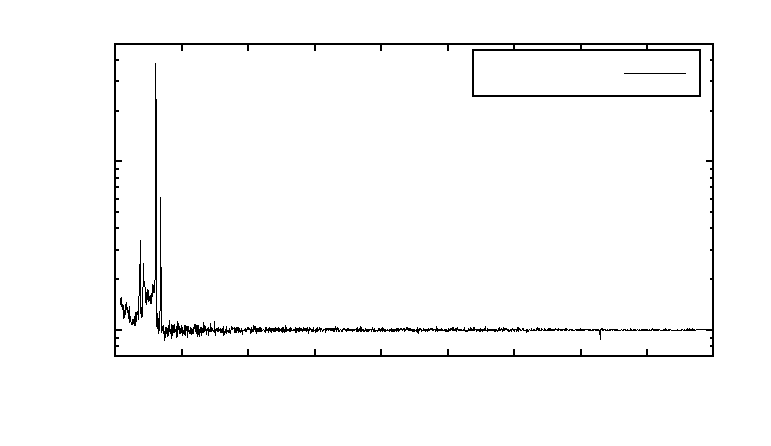
\includegraphics{kryptonit-spec-back-var}}%
    \gplfronttext
  \end{picture}%
\endgroup

				\caption{}
				\label{fig:kryptonit-var1}
			\end{subfigure}

			\begin{subfigure}[b]{\textwidth}
				\centering
				% GNUPLOT: LaTeX picture with Postscript
\begingroup
  \makeatletter
  \providecommand\color[2][]{%
    \GenericError{(gnuplot) \space\space\space\@spaces}{%
      Package color not loaded in conjunction with
      terminal option `colourtext'%
    }{See the gnuplot documentation for explanation.%
    }{Either use 'blacktext' in gnuplot or load the package
      color.sty in LaTeX.}%
    \renewcommand\color[2][]{}%
  }%
  \providecommand\includegraphics[2][]{%
    \GenericError{(gnuplot) \space\space\space\@spaces}{%
      Package graphicx or graphics not loaded%
    }{See the gnuplot documentation for explanation.%
    }{The gnuplot epslatex terminal needs graphicx.sty or graphics.sty.}%
    \renewcommand\includegraphics[2][]{}%
  }%
  \providecommand\rotatebox[2]{#2}%
  \@ifundefined{ifGPcolor}{%
    \newif\ifGPcolor
    \GPcolorfalse
  }{}%
  \@ifundefined{ifGPblacktext}{%
    \newif\ifGPblacktext
    \GPblacktexttrue
  }{}%
  % define a \g@addto@macro without @ in the name:
  \let\gplgaddtomacro\g@addto@macro
  % define empty templates for all commands taking text:
  \gdef\gplbacktext{}%
  \gdef\gplfronttext{}%
  \makeatother
  \ifGPblacktext
    % no textcolor at all
    \def\colorrgb#1{}%
    \def\colorgray#1{}%
  \else
    % gray or color?
    \ifGPcolor
      \def\colorrgb#1{\color[rgb]{#1}}%
      \def\colorgray#1{\color[gray]{#1}}%
      \expandafter\def\csname LTw\endcsname{\color{white}}%
      \expandafter\def\csname LTb\endcsname{\color{black}}%
      \expandafter\def\csname LTa\endcsname{\color{black}}%
      \expandafter\def\csname LT0\endcsname{\color[rgb]{1,0,0}}%
      \expandafter\def\csname LT1\endcsname{\color[rgb]{0,1,0}}%
      \expandafter\def\csname LT2\endcsname{\color[rgb]{0,0,1}}%
      \expandafter\def\csname LT3\endcsname{\color[rgb]{1,0,1}}%
      \expandafter\def\csname LT4\endcsname{\color[rgb]{0,1,1}}%
      \expandafter\def\csname LT5\endcsname{\color[rgb]{1,1,0}}%
      \expandafter\def\csname LT6\endcsname{\color[rgb]{0,0,0}}%
      \expandafter\def\csname LT7\endcsname{\color[rgb]{1,0.3,0}}%
      \expandafter\def\csname LT8\endcsname{\color[rgb]{0.5,0.5,0.5}}%
    \else
      % gray
      \def\colorrgb#1{\color{black}}%
      \def\colorgray#1{\color[gray]{#1}}%
      \expandafter\def\csname LTw\endcsname{\color{white}}%
      \expandafter\def\csname LTb\endcsname{\color{black}}%
      \expandafter\def\csname LTa\endcsname{\color{black}}%
      \expandafter\def\csname LT0\endcsname{\color{black}}%
      \expandafter\def\csname LT1\endcsname{\color{black}}%
      \expandafter\def\csname LT2\endcsname{\color{black}}%
      \expandafter\def\csname LT3\endcsname{\color{black}}%
      \expandafter\def\csname LT4\endcsname{\color{black}}%
      \expandafter\def\csname LT5\endcsname{\color{black}}%
      \expandafter\def\csname LT6\endcsname{\color{black}}%
      \expandafter\def\csname LT7\endcsname{\color{black}}%
      \expandafter\def\csname LT8\endcsname{\color{black}}%
    \fi
  \fi
  \setlength{\unitlength}{0.0500bp}%
  \begin{picture}(7086.00,3968.00)%
    \gplgaddtomacro\gplbacktext{%
      \csname LTb\endcsname%
      \put(814,955){\makebox(0,0)[r]{\strut{}$10^{0}$}}%
      \put(814,2572){\makebox(0,0)[r]{\strut{}$10^{1}$}}%
      \put(1520,484){\makebox(0,0){\strut{} 60}}%
      \put(2669,484){\makebox(0,0){\strut{} 80}}%
      \put(3818,484){\makebox(0,0){\strut{} 100}}%
      \put(4966,484){\makebox(0,0){\strut{} 120}}%
      \put(6115,484){\makebox(0,0){\strut{} 140}}%
      \put(176,2203){\rotatebox{-270}{\makebox(0,0){\strut{}Intensität}}}%
      \put(3817,154){\makebox(0,0){\strut{}$E \ [\unit{keV}]$}}%
    }%
    \gplgaddtomacro\gplfronttext{%
      \csname LTb\endcsname%
      \put(2398,3420){\makebox(0,0)[r]{\strut{}Messwerte}}%
    }%
    \gplbacktext
    \put(0,0){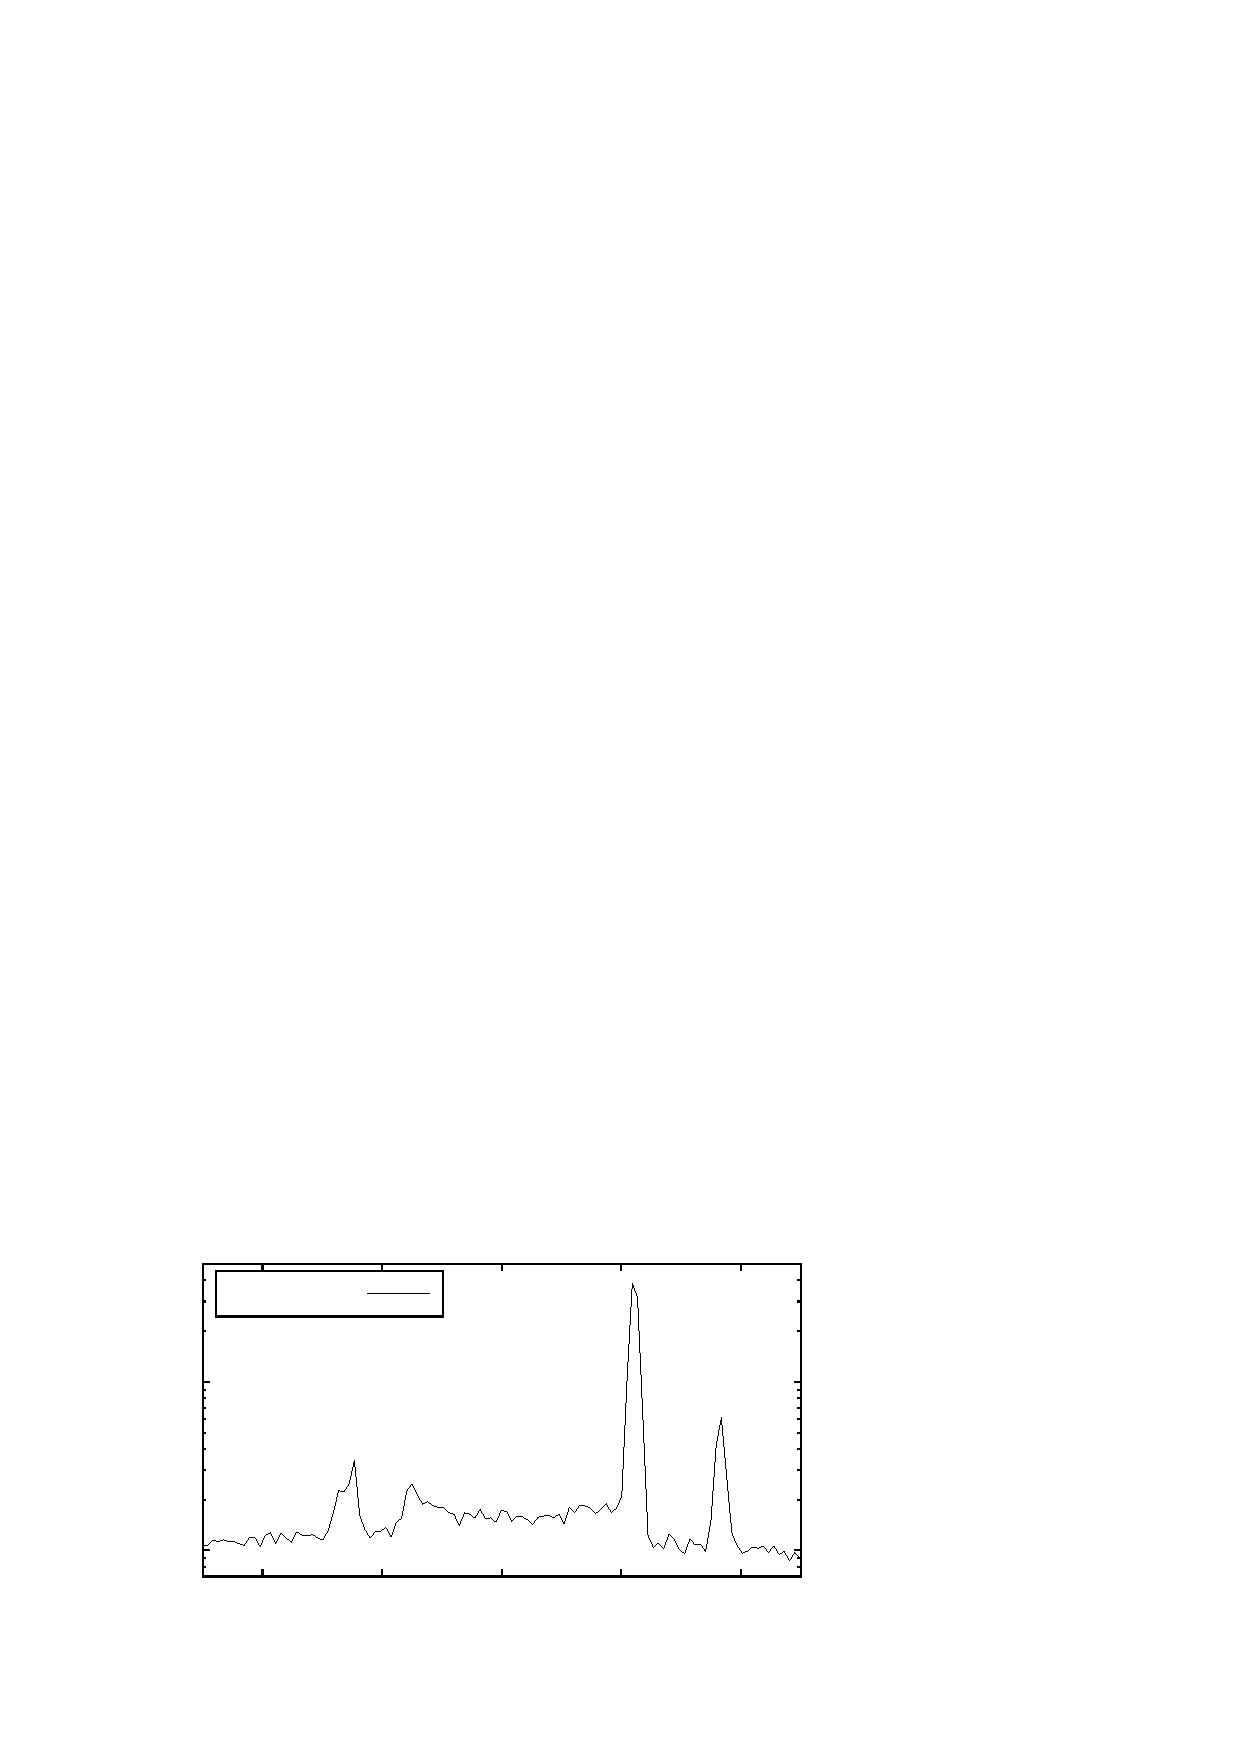
\includegraphics{kryptonit-spec-back}}%
    \gplfronttext
  \end{picture}%
\endgroup

				\caption{}
				\label{fig:kryptonit-var2}
			\end{subfigure}
			\caption{kalibriertes $\gamma$-Spektrum einer unbekannten Probe im Abstand $d=20\unit{cm}$ aufgenommen durch den HP-Ge-Detektor}
			\label{fig:kryptonit}
		\end{figure}
	
	\FloatBarrier
	% subsection kryptonit

% section messwerte